%
% Setup.tex
%
% LulzBot Mini User Manual
%
% Copyright (C) 2014 Aleph Objects, Inc.
%
% This document is licensed under the Creative Commons Attribution 4.0
% International Public License (CC BY-SA 4.0) by Aleph Objects, Inc.
%
%
%%%% This section is no longer needed, as the information to the Quick Start Guide %%%%

\section{Hardware Setup}
\begin{enumerate}
\item Your printer has been calibrated and tested, however, after unpacking all of the components you will need to re-mount the Y axis onto the frame and connect the bed and Y axis connectors. You will also need to re-mount the extruder tool head. Please follow the steps completely to make certain that the extruder tool head and Y axis are re-mounted correctly. You will then be on your way to your first print. Use Fig. \ref{fig:axes} to see which direction the three axes move, as the following instructions will reference the X, Y, and Z axes.

\begin{figure}[H]
\centering
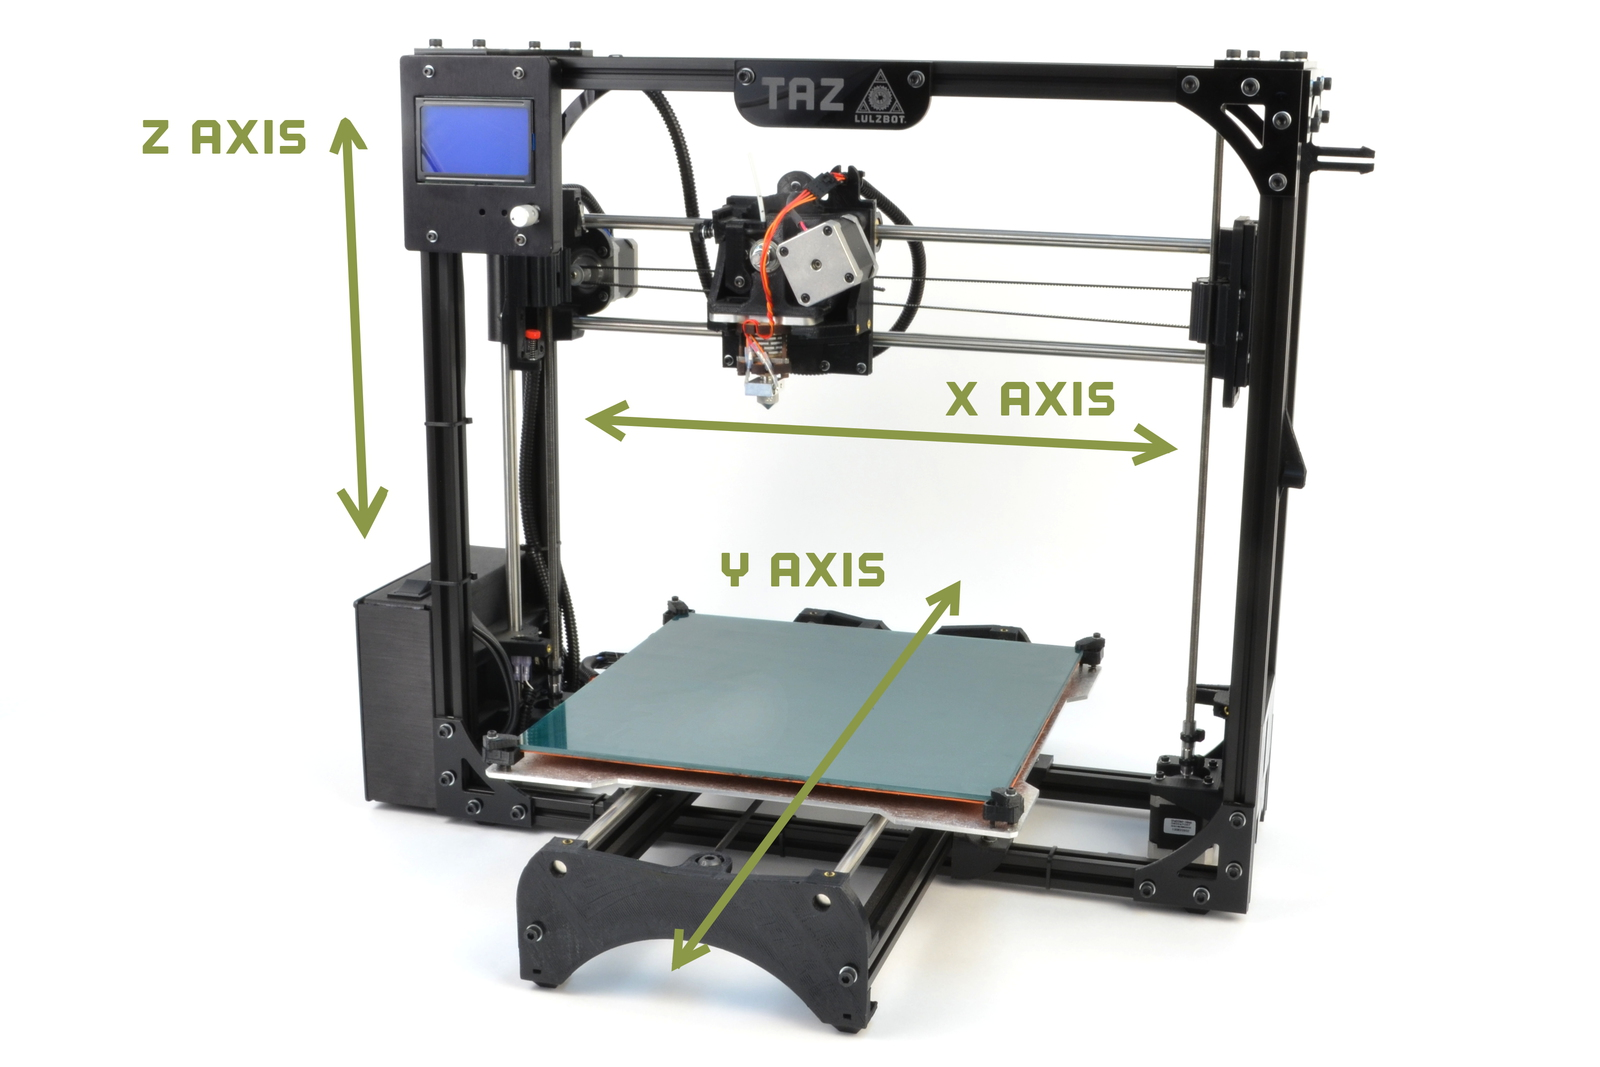
\includegraphics[keepaspectratio=true,angle=0,height=0.4\textheight,width=1.0\textwidth]{axes.JPG}
\caption{Axes movement directions}
\label{fig:axes}
\end{figure}

\item Place the Mini on a flat and level surface. 


\item \textcolor{red}{Before proceeding make sure that the four red shipping clamps on the Z axis smooth rods have been removed.}

\item Move the X axis carriage to the center of the smooth rods. If you have not already done so, remove the foam from between the X axis carriage and the left hand X axis end. Locate and remove, with the included 2.5mm hex driver, the tool head M3 screw in top center of the X axis carriage (Fig. \ref{fig:tool_head_screw}, page \pageref{fig:tool_head_screw}). Place the extruder tool head mount onto the X axis carriage bottom first. The extruder mount will slide into the bottom portion of the carriage and self center (Fig. \ref{fig:tool_head_placement}, page \pageref{fig:tool_head_placement}).Make sure that the tool head mount is fully seated. Use the 2.5mm driver and the previously removed M3 screw to secure the extruder tool head onto the X axis carriage.
\begin{figure}[hp]
\centering
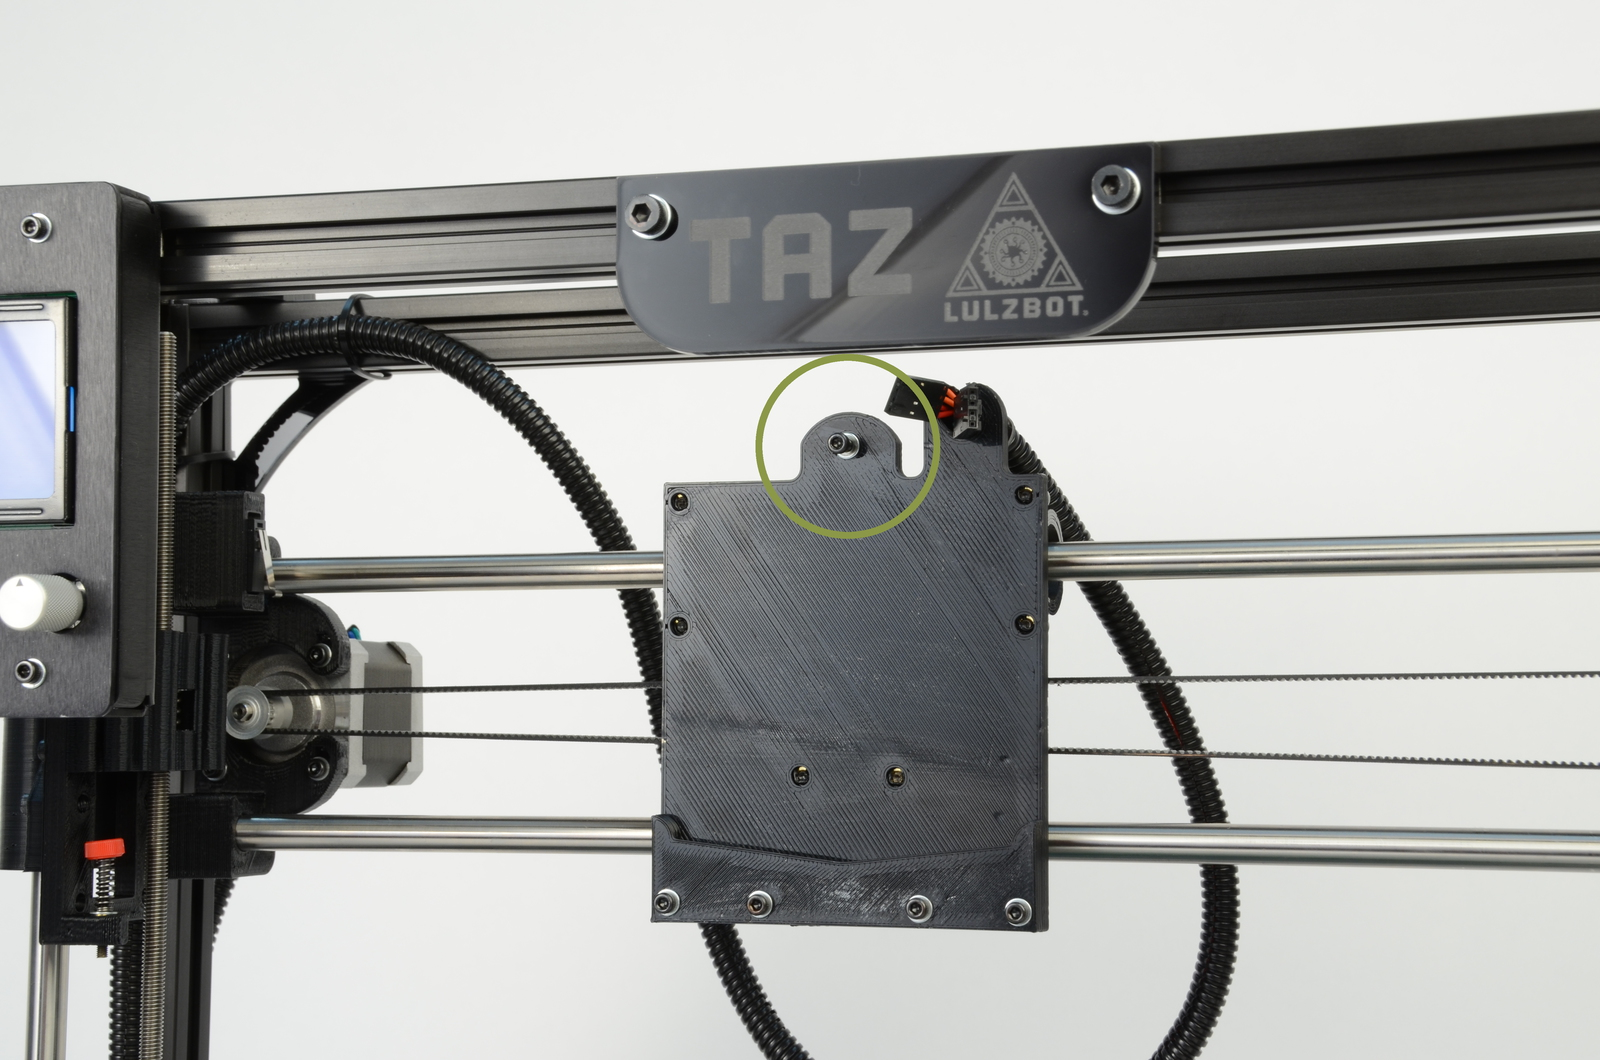
\includegraphics[keepaspectratio=true,angle=0,height=0.4\textheight,width=1.0\textwidth]{tool_head_screw.JPG}
\caption{Remove the tool head screw}
\label{fig:tool_head_screw}
\end{figure}

\begin{figure}[hp]
\centering
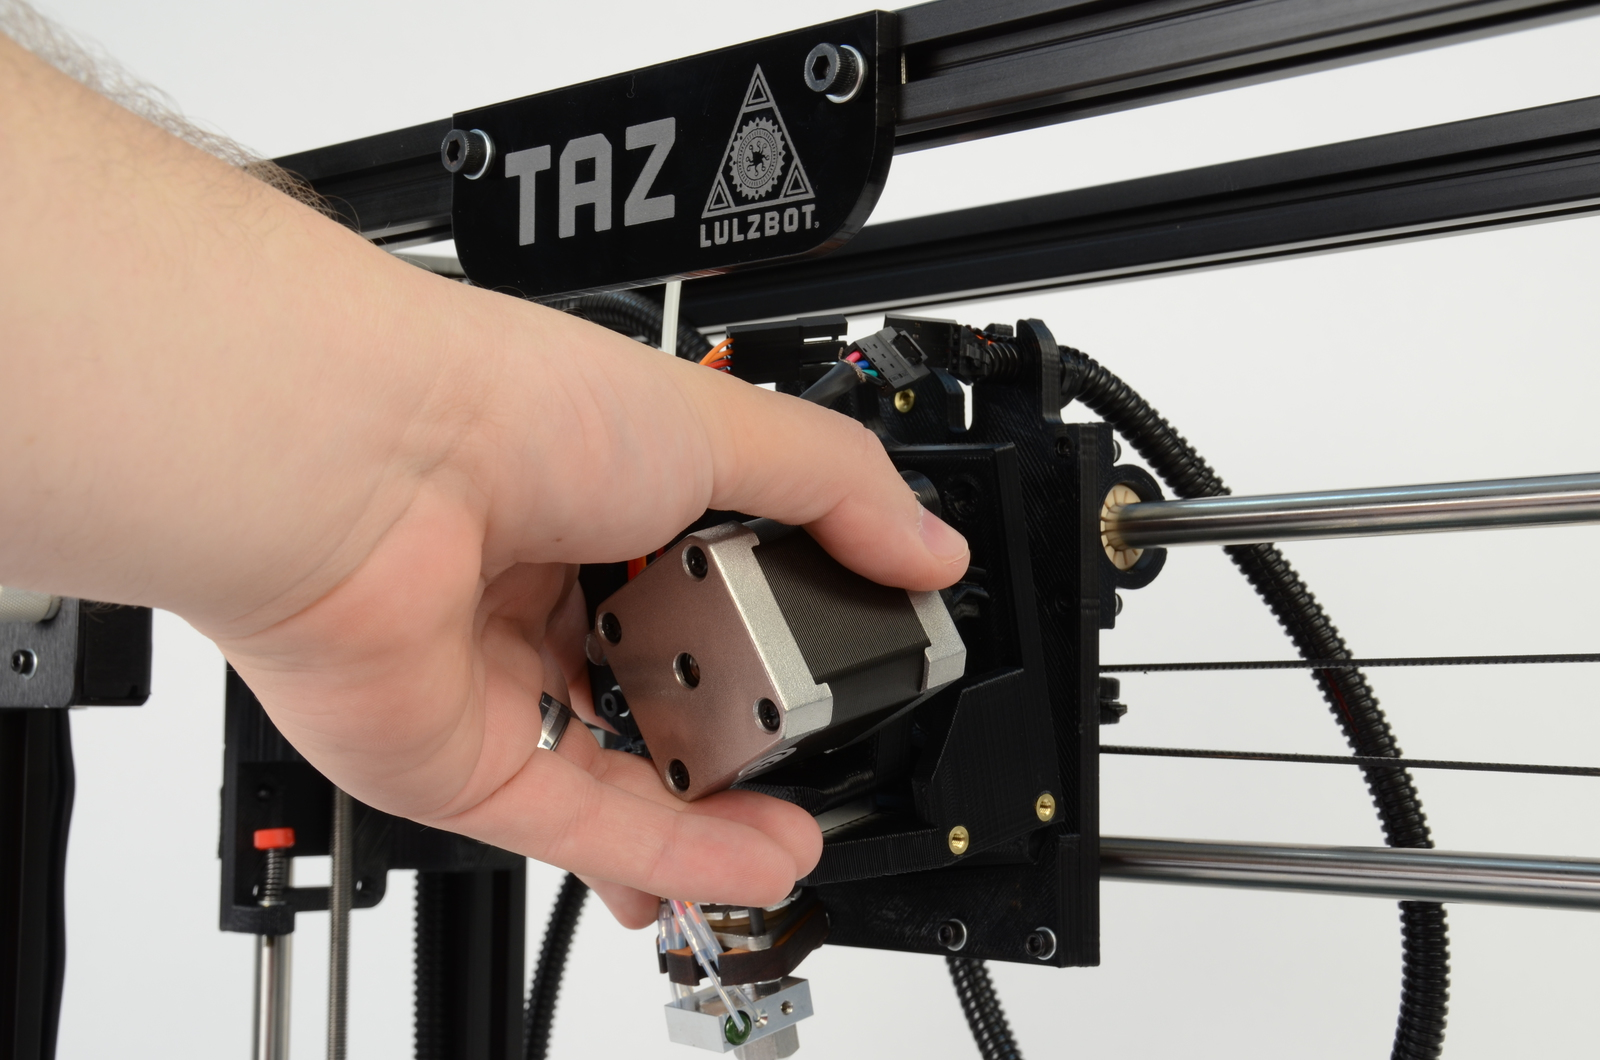
\includegraphics[keepaspectratio=true,angle=0,height=0.4\textheight,width=1.0\textwidth]{tool_head_placement.JPG}
\caption{Mount the extruder tool head}
\label{fig:tool_head_placement}
\end{figure}

\begin{figure}[hp]
\centering
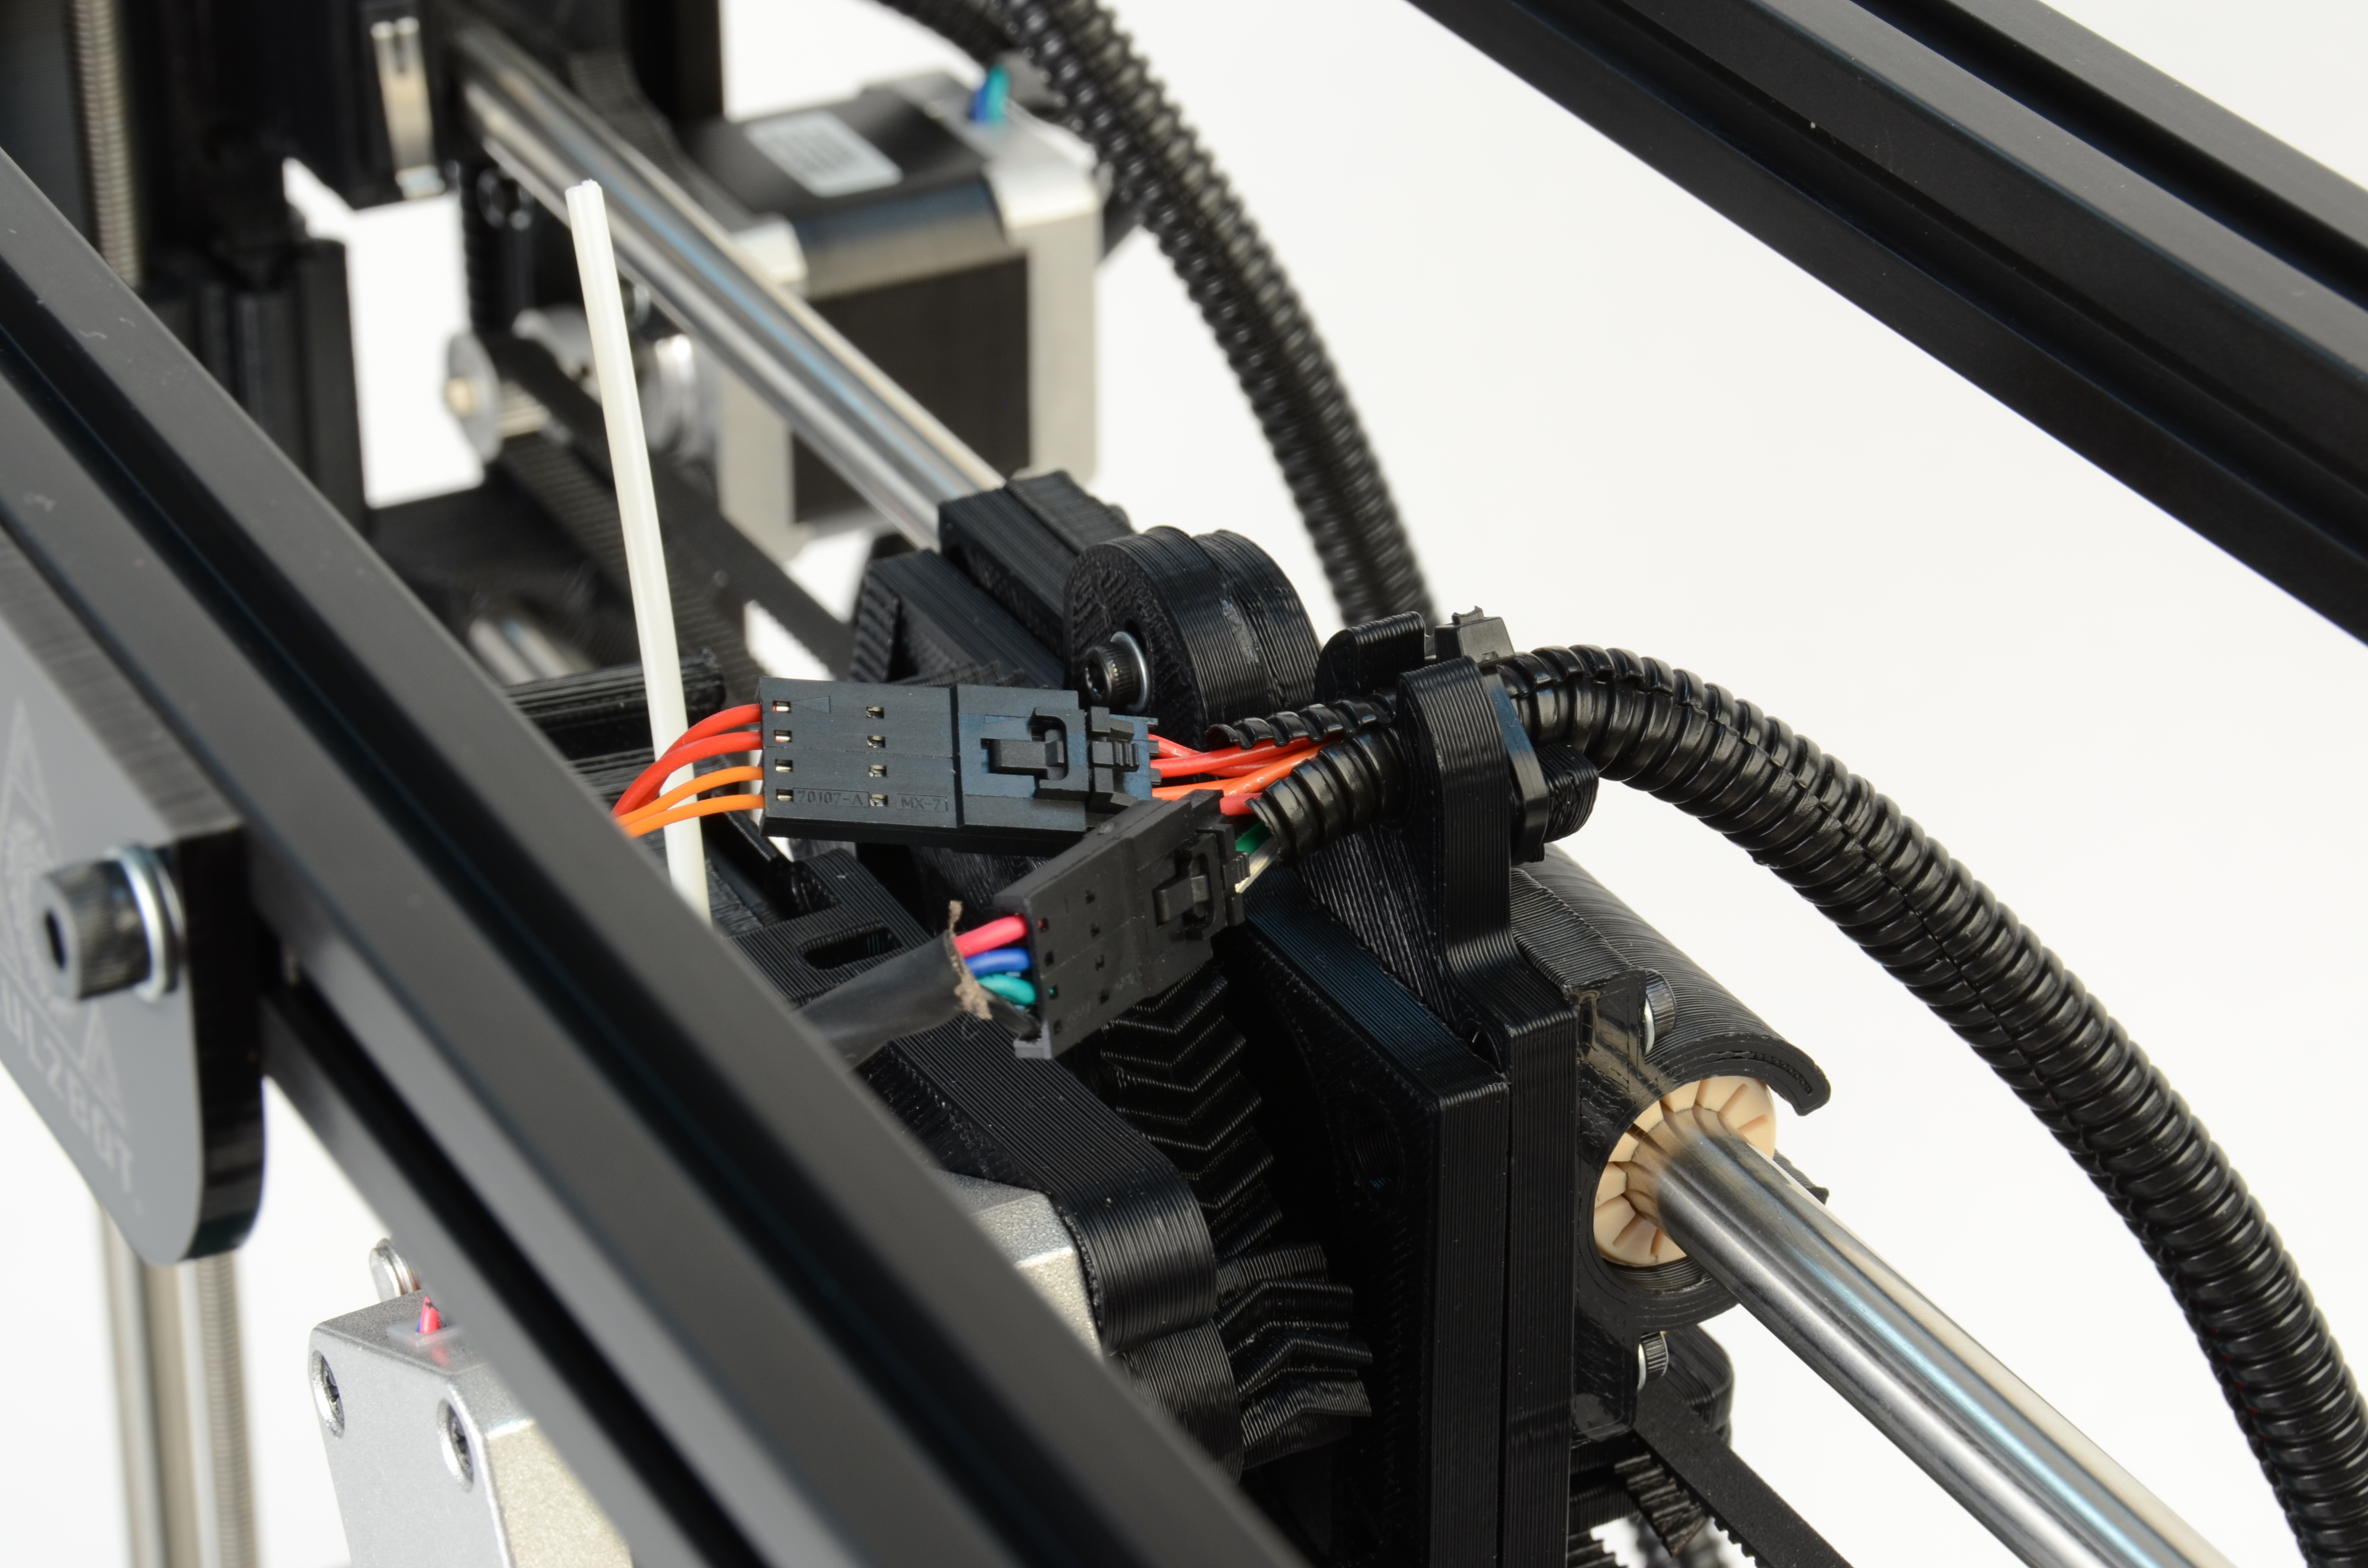
\includegraphics[keepaspectratio=true,angle=0,height=0.4\textheight,width=1.0\textwidth]{tool_head_connectors.JPG}
\caption{Connect the two tool head connectors}
\label{fig:tool_head_connectors}
\end{figure}

\item Connect the stepper motor and the hot end to the existing wiring harness located at the top of the X axis carriage. Connect the extruder assemblies' 4-pin connectors: match the orange/red wire connector pair for the hot end and the mixed color wired connector pair for the extruder motor (Fig. \ref{fig:tool_head_connectors}, page \pageref{fig:tool_head_connectors}). Connect the matching pairs together so they lock and click.

\item Now that the Y axis is mounted and the extruder tool head is installed you should set your printer on a stable, flat, and level surface large enough for extra space around the printer. Make sure your printer work space is clear of anything that could obstruct the movement of the printer. Move the Y axis to the back of the printer to ensure unobstructed movement of that axis. \textcolor{red}{Make sure there are no flammable fabrics or liquids near the printer space}. It is also best to not put your printer near a drafty window or air conditioner vent.

\index{power supply}
\index{USB cable}
\item Unwrap the power supply and USB cables.

\textcolor{red}{MAKE SURE THE POWER SUPPLY IS COMPLETELY UNPLUGGED BEFORE MOVING ON TO THE NEXT STEP}.

\index{electronics receptacles}
\item Locate the power supply and USB receptacles along the back of the Mini electronics enclosure
(Fig. \ref{fig:electronics_plugs}, page \pageref{fig:electronics_plugs}). Locate the power supply and the included AC power cable (Fig. \ref{fig:power_supply}, page \pageref{fig:power_supply}). Locate the DC power cable plug on the power supply. Connect the DC locking plug into the DC connector on the Mini electronics enclosure (Fig. \ref{fig:ps_plug}, page \pageref{fig:ps_plug}). The plug is keyed which may require rotating the plug until the keys line up and the plug can be pushed in. Once you have pushed in the plug turn the locking sleeve clockwise until it is tight against the electronics enclosure (Fig. \ref{fig:electronics_plugs_plugged-in}, page \pageref{fig:electronics_plugs_plugged-in}).
%\begin{figure}[hbt]
\begin{figure}[H]
\centering
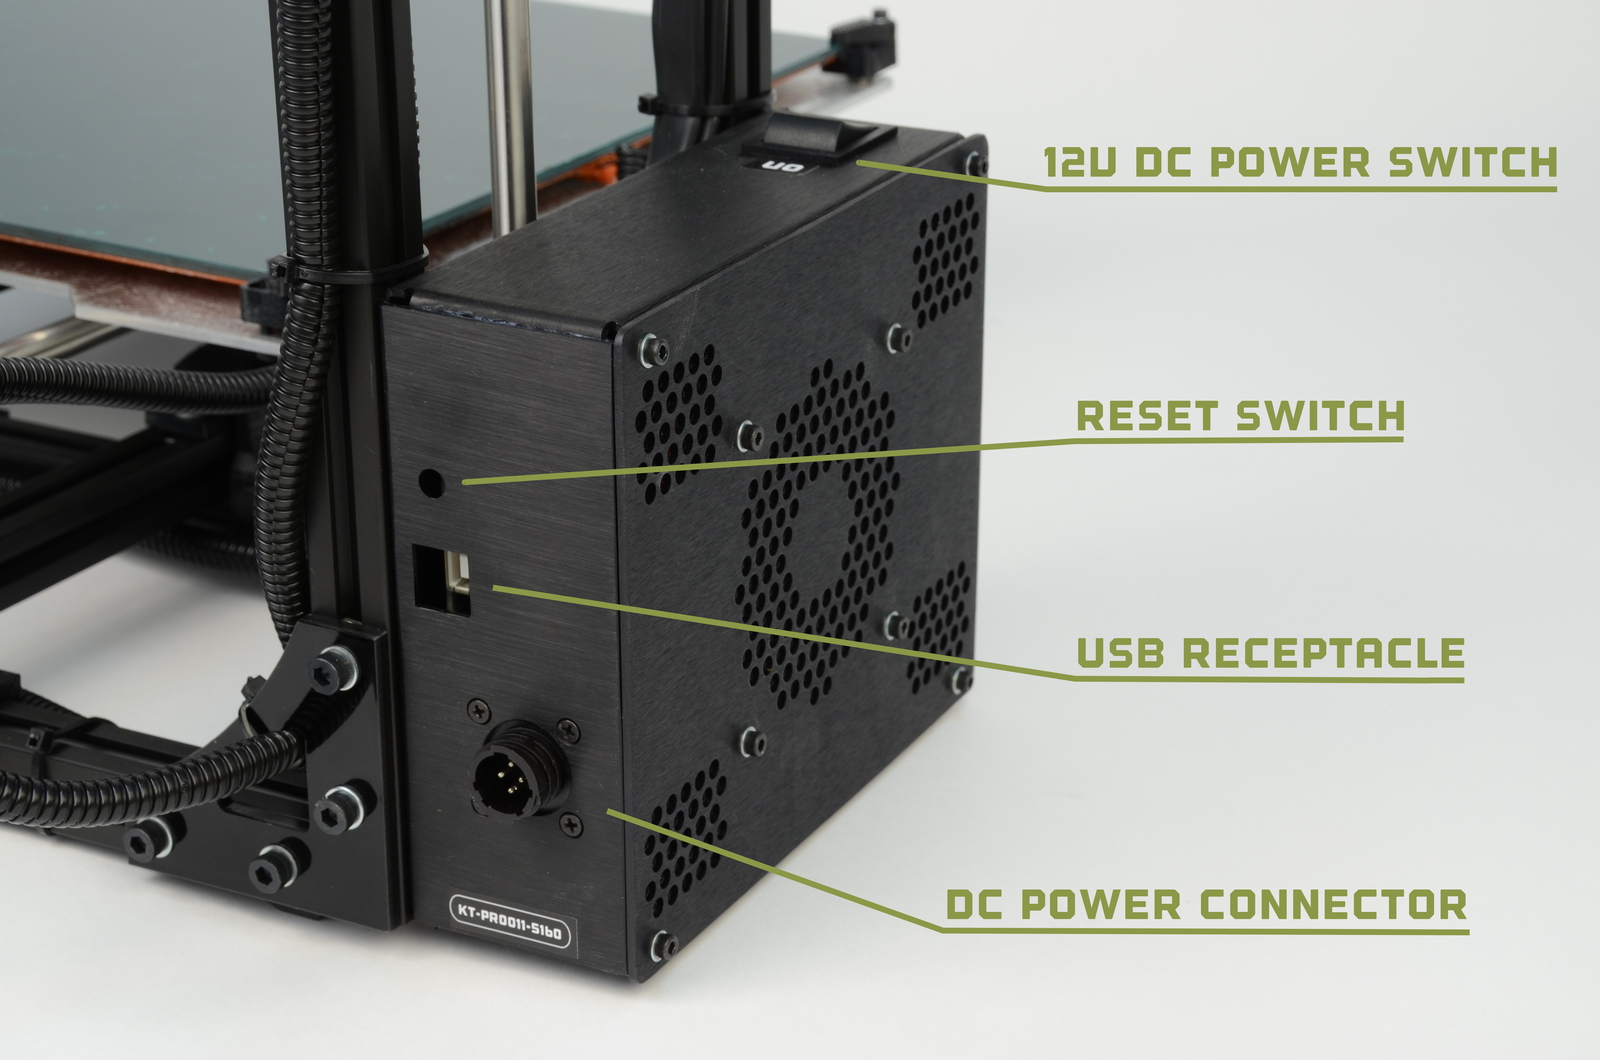
\includegraphics[keepaspectratio=true,angle=0,height=0.4\textheight,width=1.0\textwidth]{electronics_case_rec.JPG}
\caption{Power and USB receptacles}
\label{fig:electronics_plugs}
\end{figure}

%\begin{figure}[hp]
\begin{figure}[H]
\centering
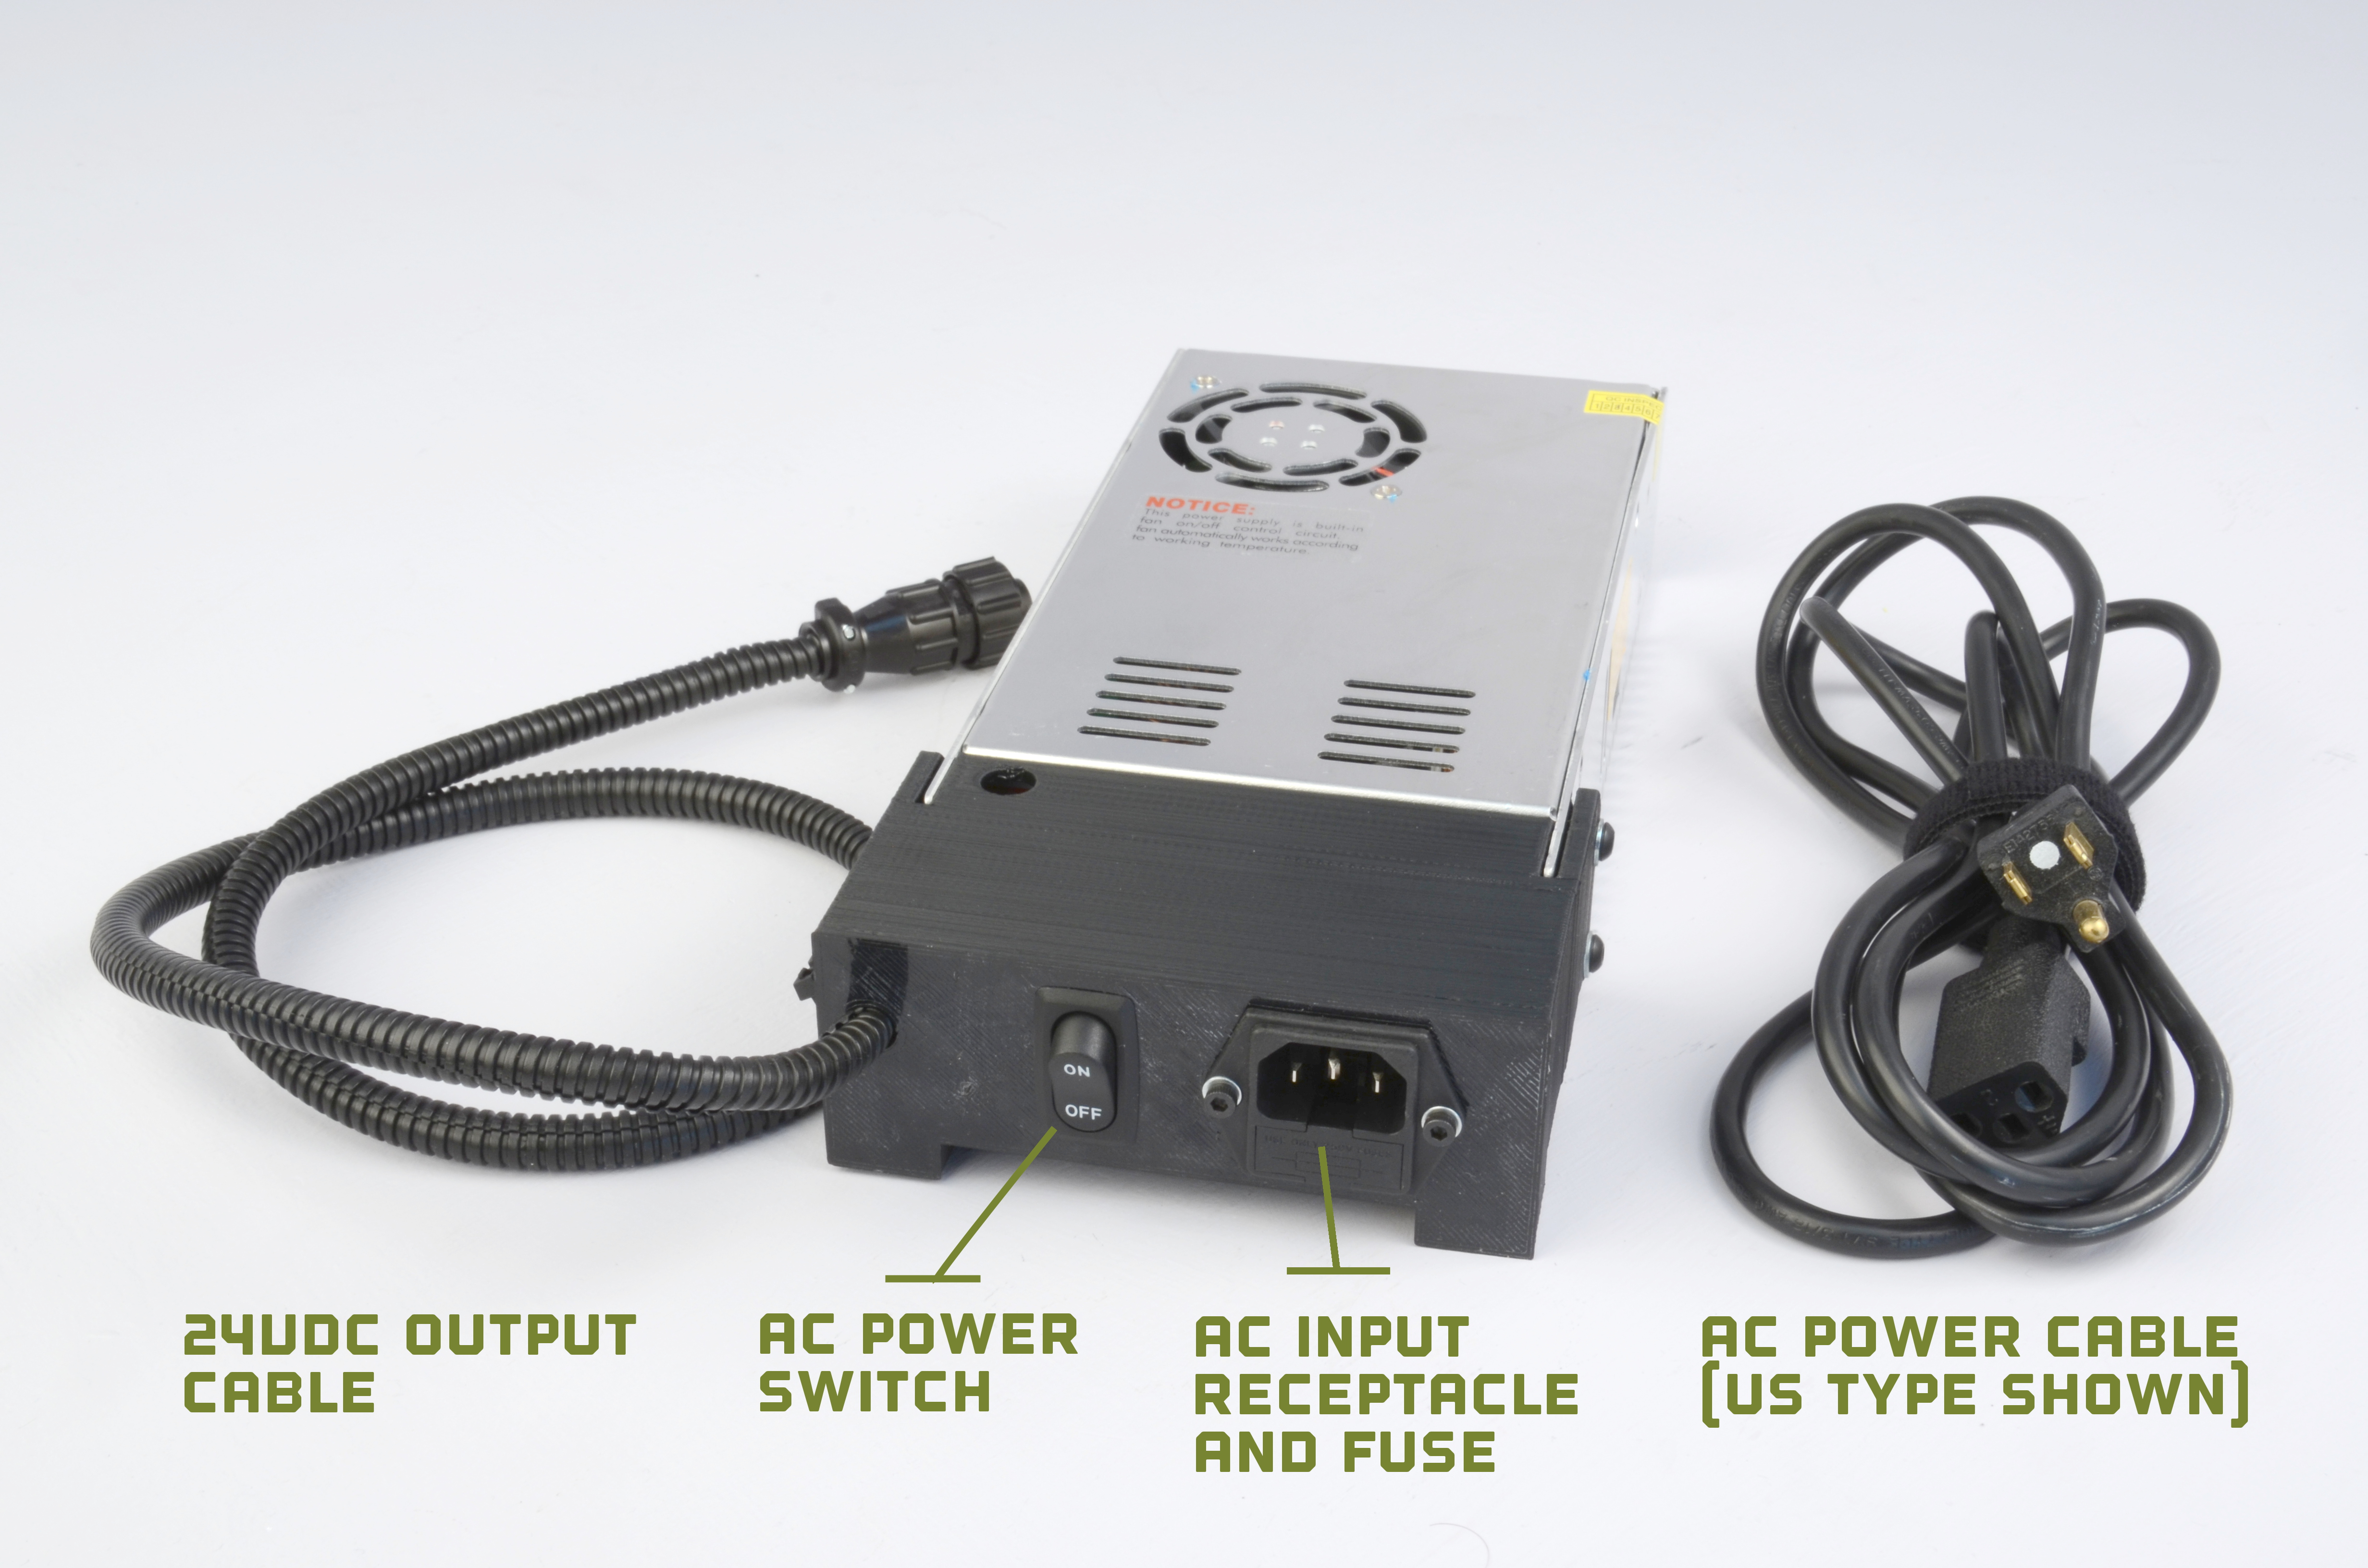
\includegraphics[keepaspectratio=true,angle=0,height=0.4\textheight,width=1.0\textwidth]{power_supply.JPG}
\caption{Power supply}
\label{fig:power_supply}
\end{figure}

%\begin{figure}[hp]
\begin{figure}[H]
\centering
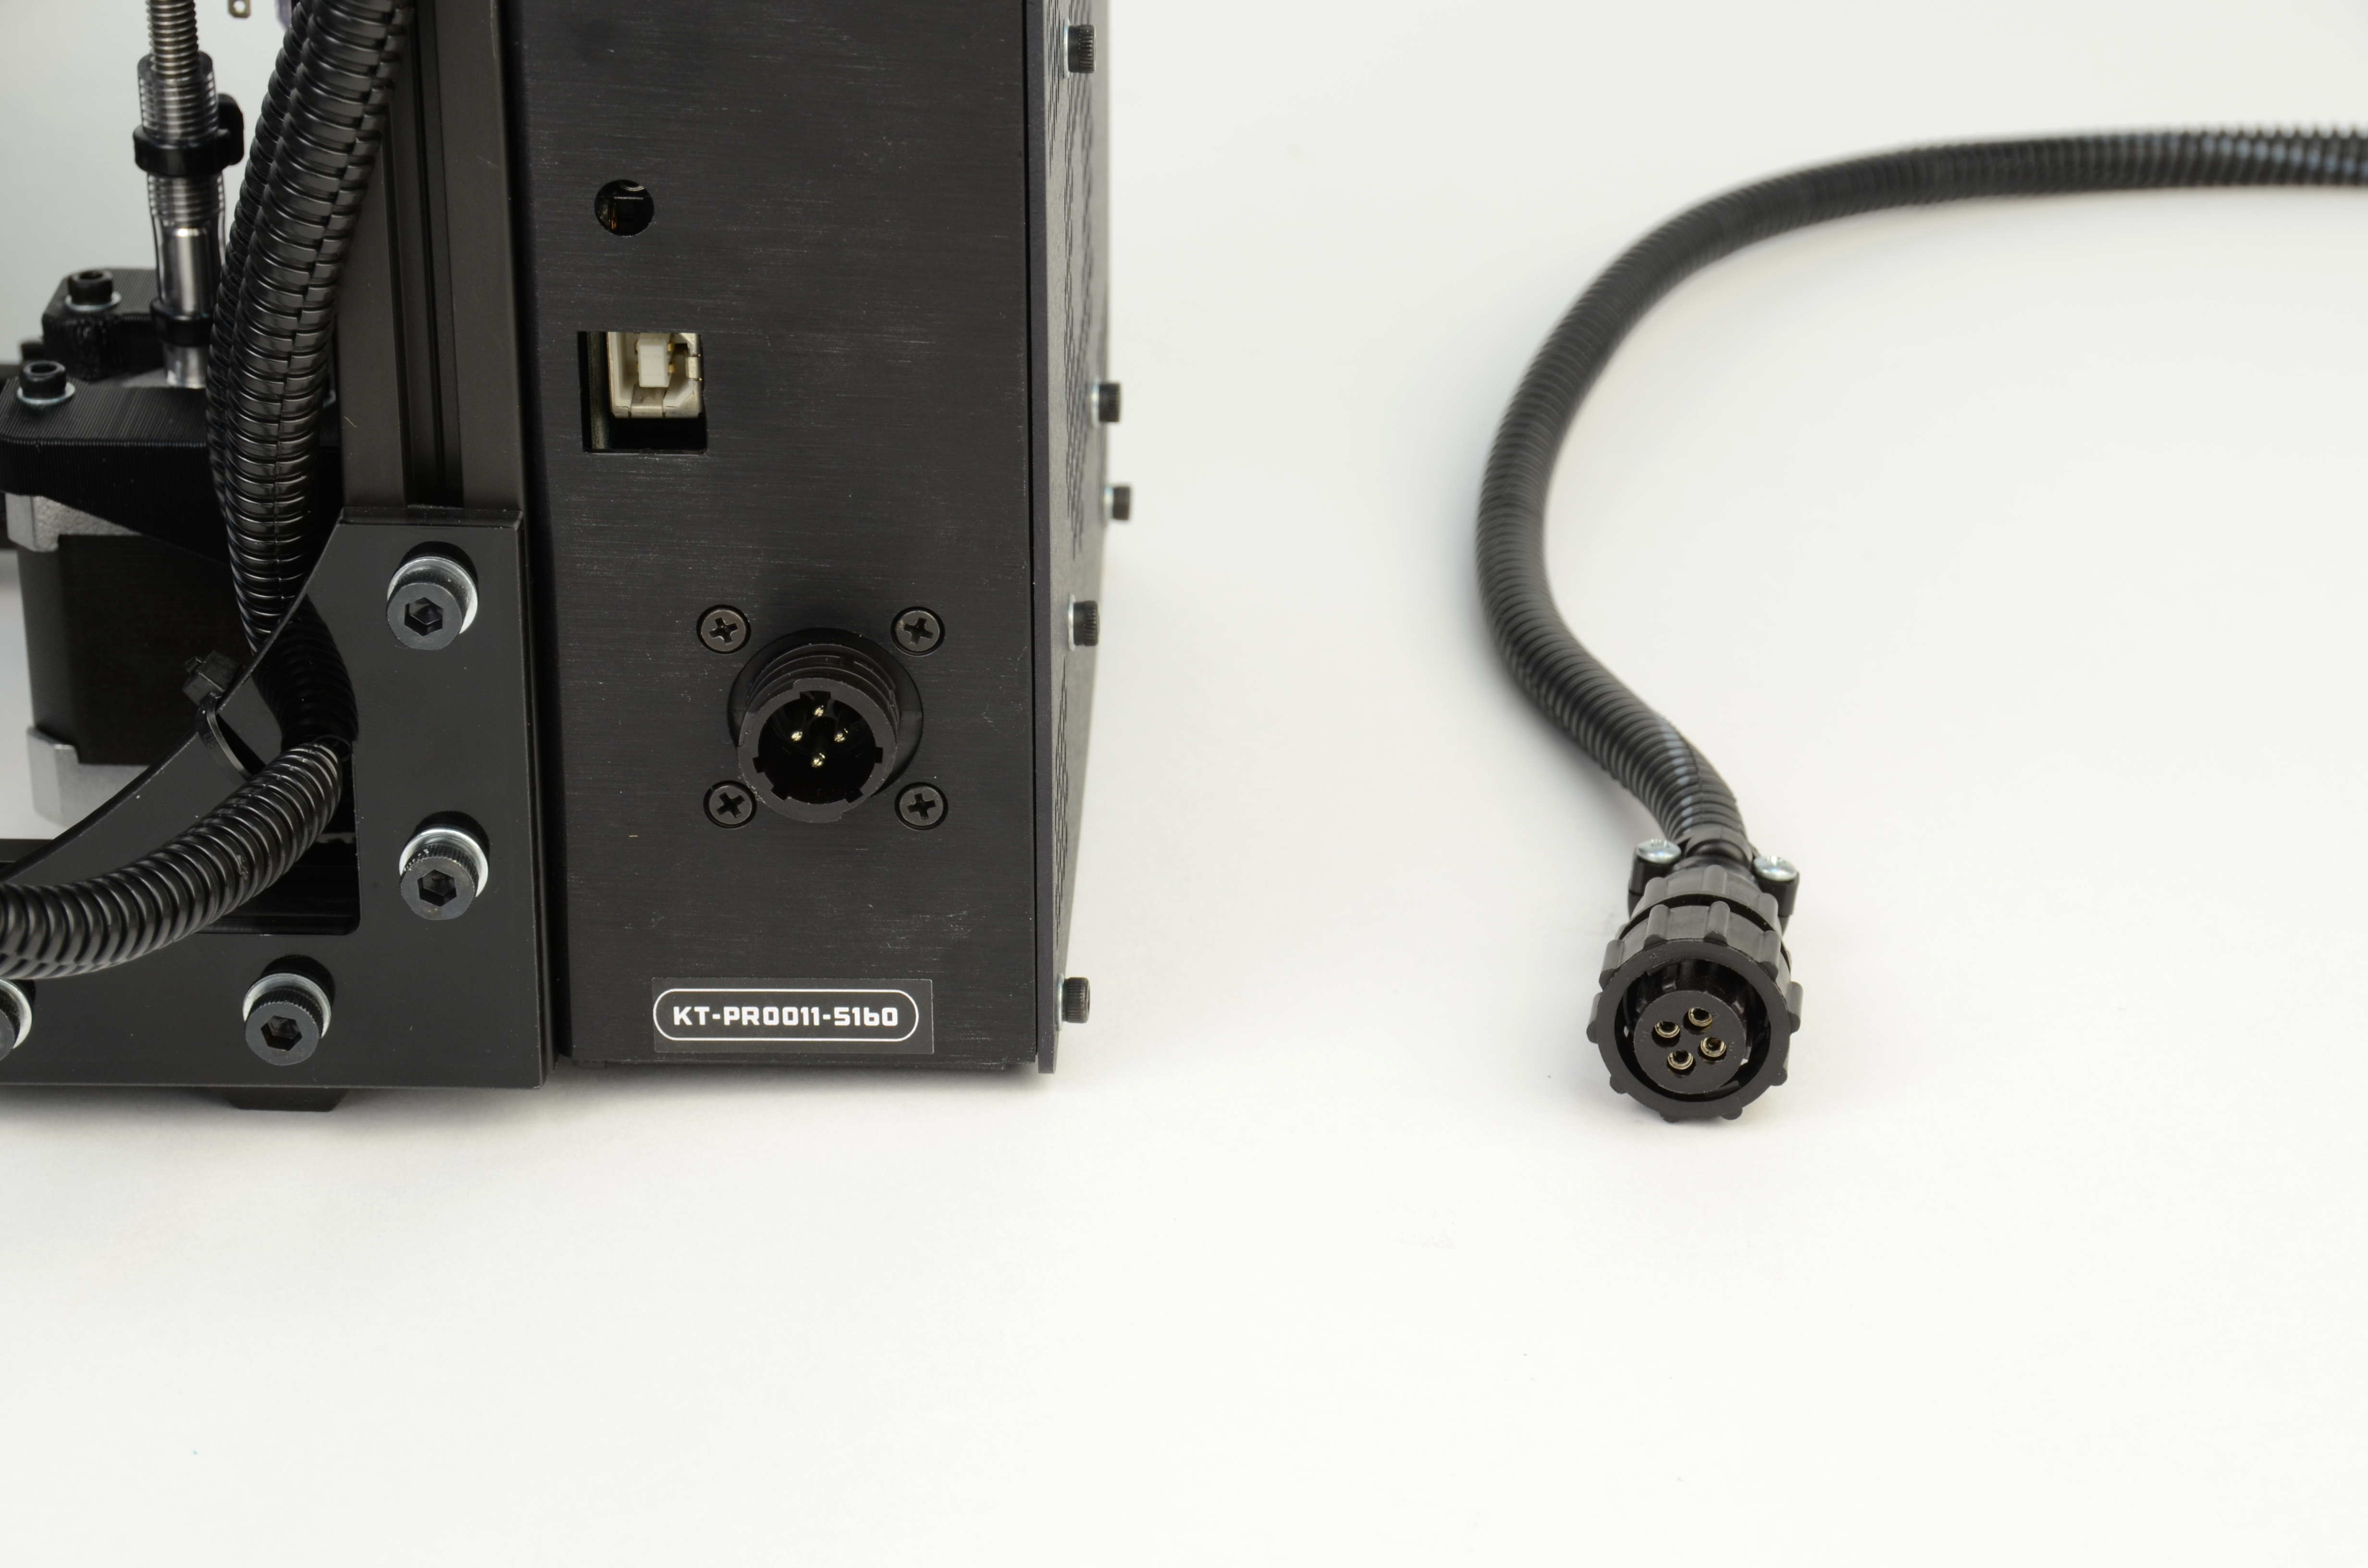
\includegraphics[keepaspectratio=true,angle=0,height=0.4\textheight,width=1.0\textwidth]{electronics_DC_connector.JPG}
\caption{24V DC Power supply plug and receptacle}
\label{fig:ps_plug}
\end{figure}

%\begin{figure}[hp]
\begin{figure}[H]
\centering
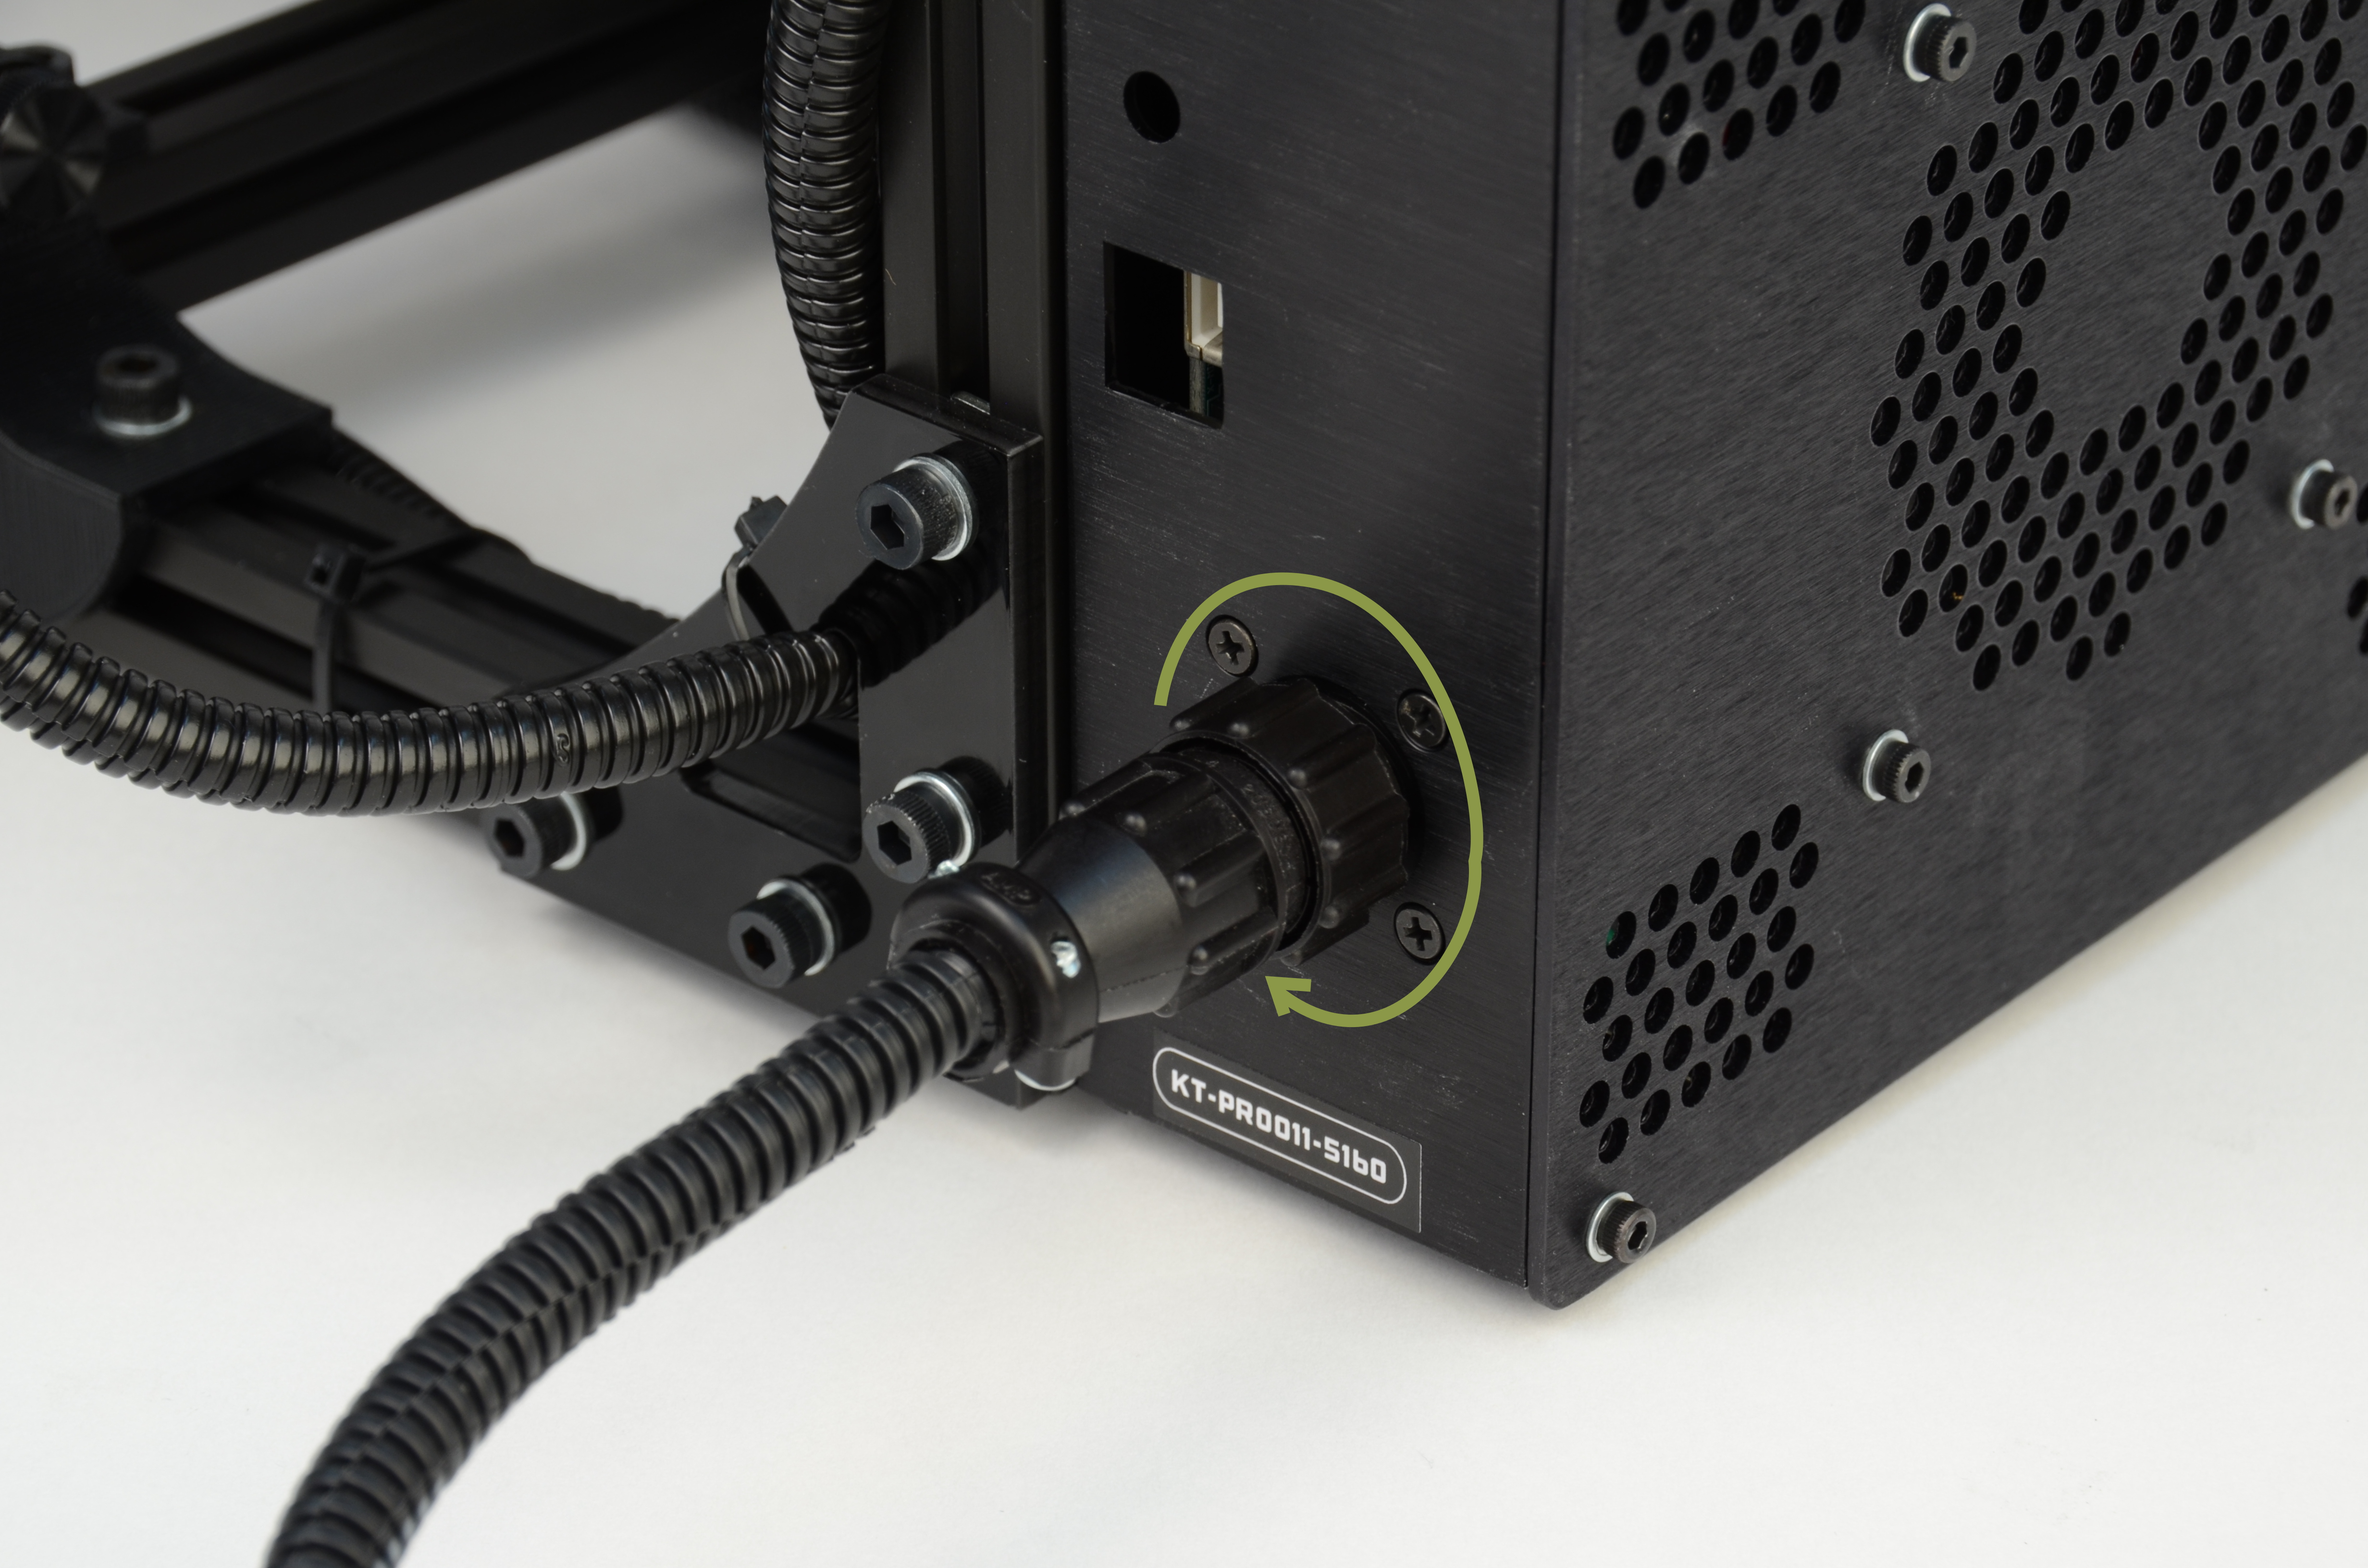
\includegraphics[keepaspectratio=true,angle=0,height=0.4\textheight,width=1.0\textwidth]{electronics_DC_connector_tight.JPG}
\caption{The power supply plug correctly plugged in}
\label{fig:electronics_plugs_plugged-in}
\end{figure}

\item Locate, on the right of the power supply, the red AC voltage switch. Depending on your location you will need to change the AC voltage switch to 115V or 230V. North America is generally 115V and the majority of other regions are 230V. You can find general voltage by country at \texttt{wikipedia.org/wiki/Mains\_electricity\_by\_country}. Make sure that when plugging in the AC power cable it is directly plugged into the wall and \textbf{not} into a power strip. The Mini 3D printer can potentially pull more current than the power strip will support and may lead to undesirable performance. 

\index{RAMBo}
\item Plug in the USB cable, B plug (smaller square plug) side, into the USB receptacle on the printer electronics. Plug the other end of the USB cable, (larger), into your computer.

\index{Filament Mount}
\item Rotate the Filament Mount up and into position. Firmly seat the base of the Filament Mount until it locks into place.
(Fig. \ref{fig:filament_guide}, page \pageref{fig:filament_guide}). 
%\begin{figure}[hbt]
\begin{figure}[H]
\centering
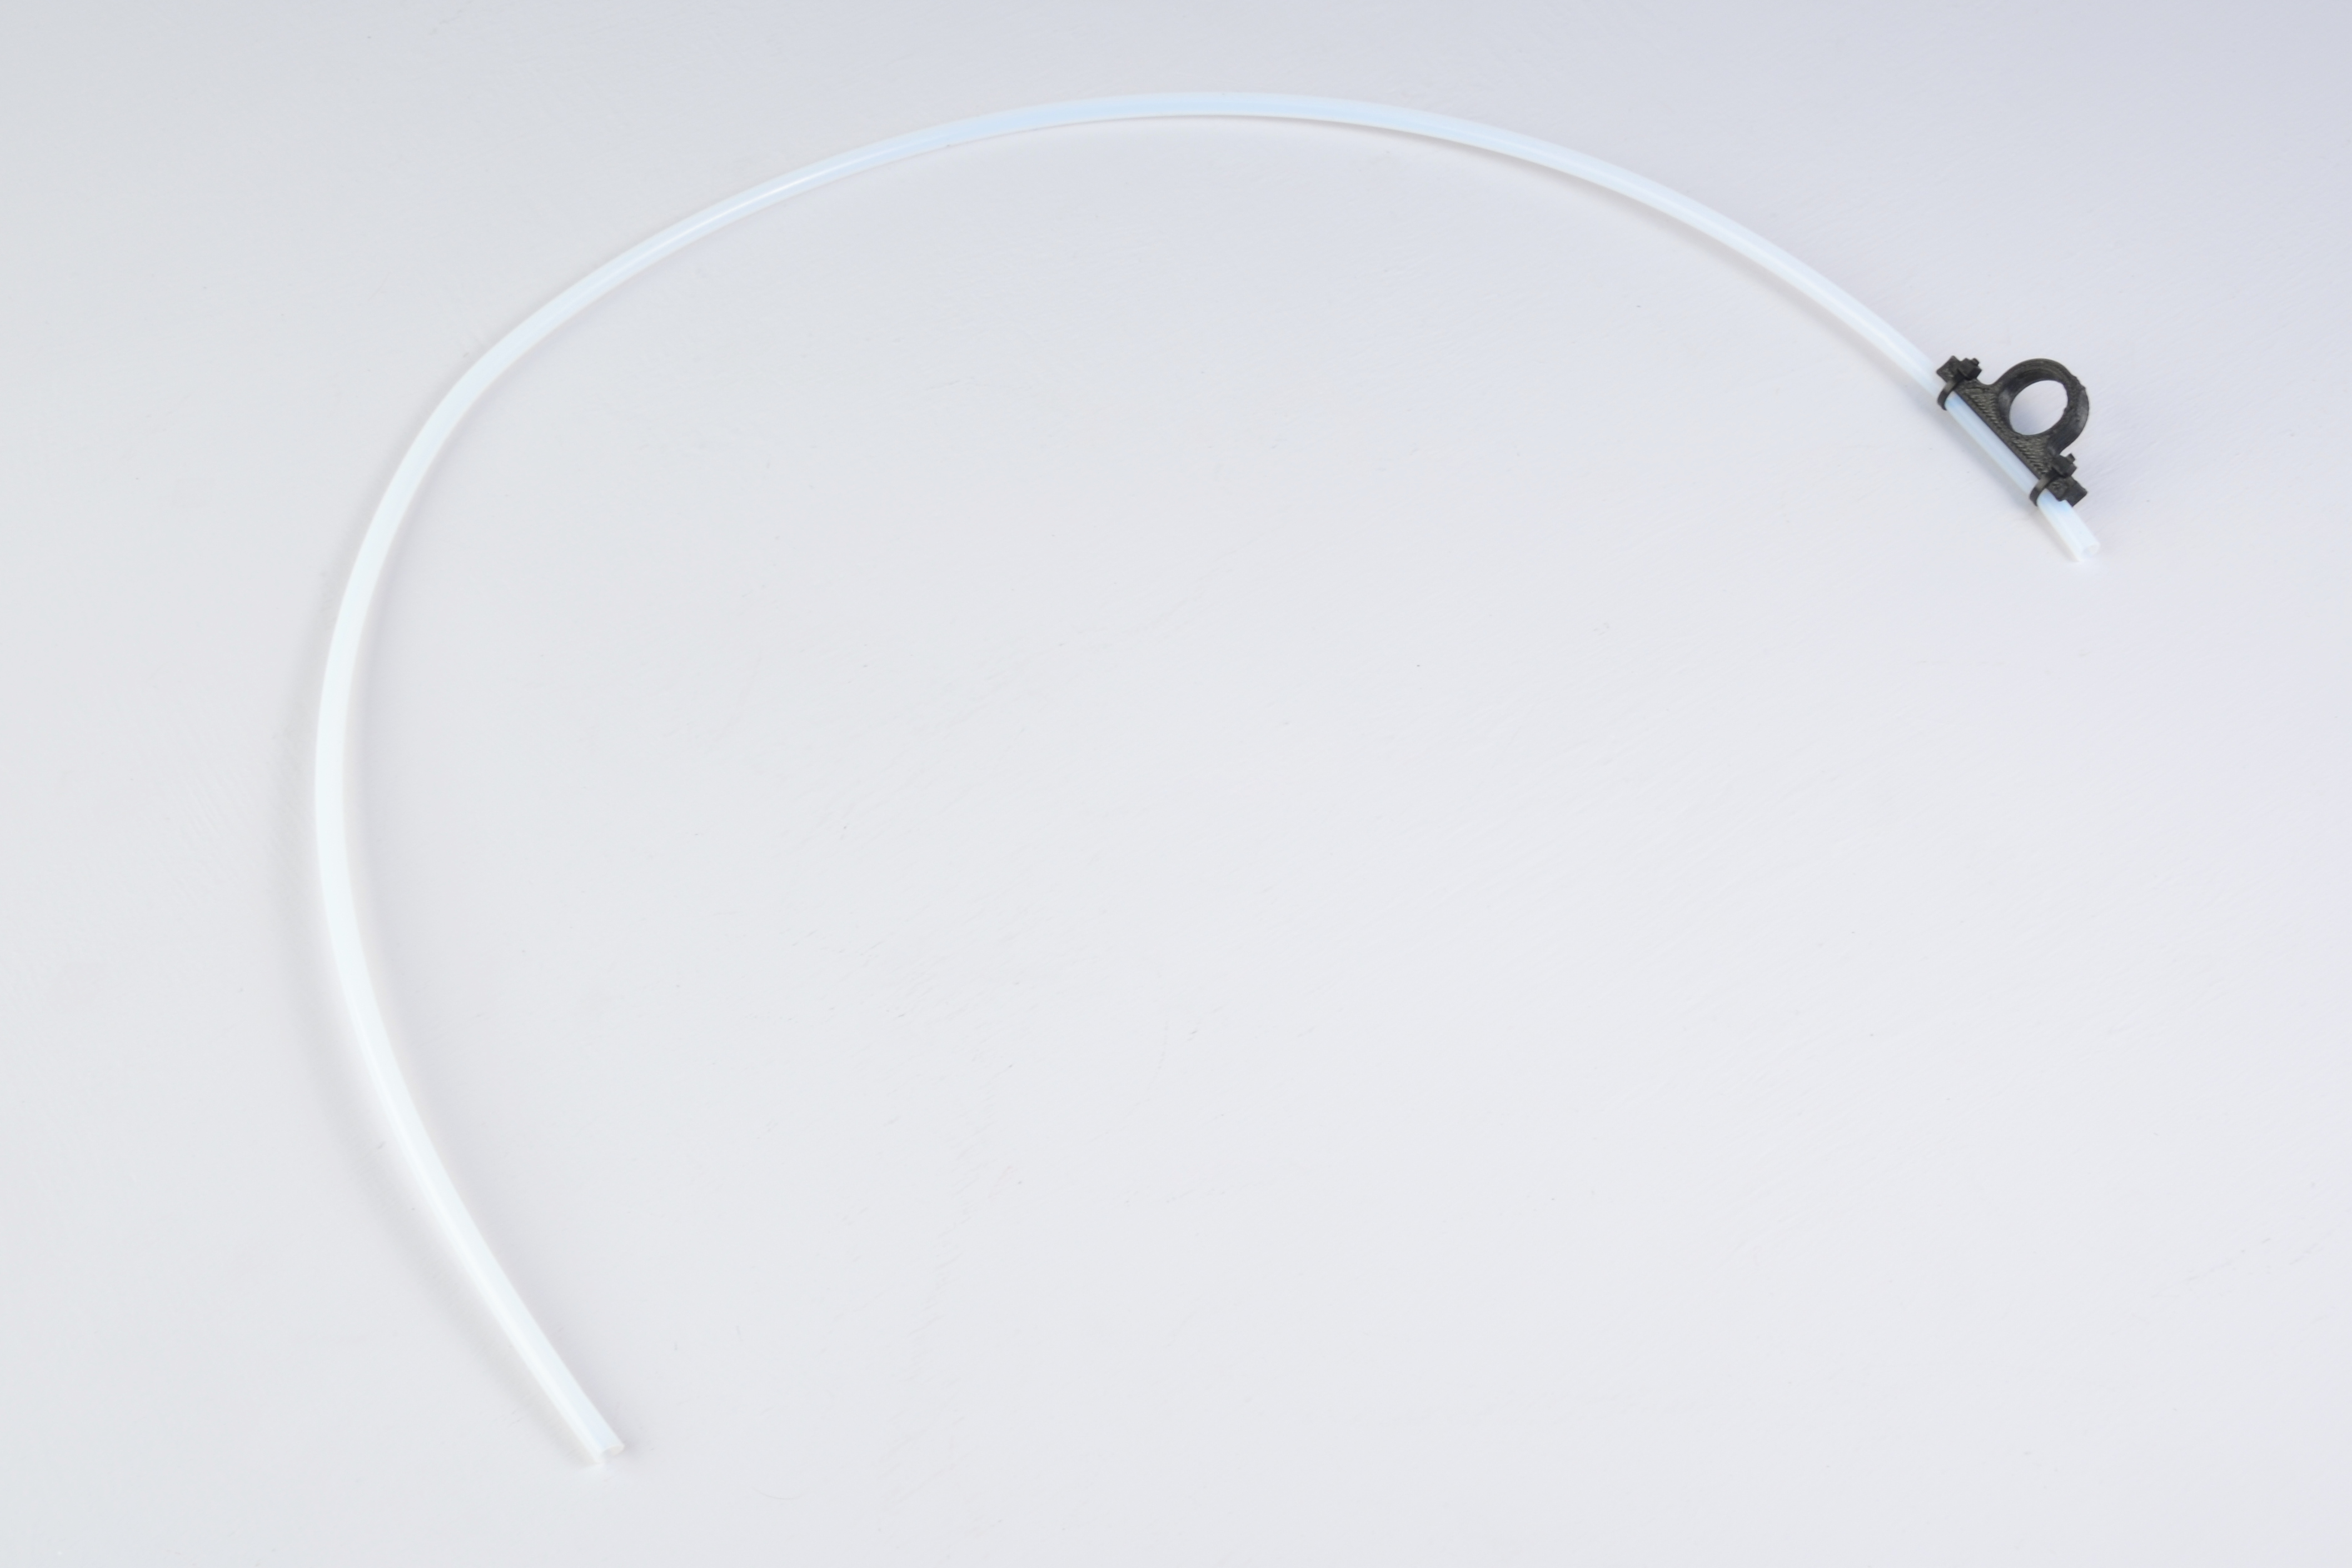
\includegraphics[keepaspectratio=true,angle=0,height=0.4\textheight,width=1.0\textwidth]{filament_guide.JPG}
\caption{Filament Guide}
\label{fig:filament_guide}
\end{figure}

%\begin{figure}[hbt]
\begin{figure}[H]
\centering
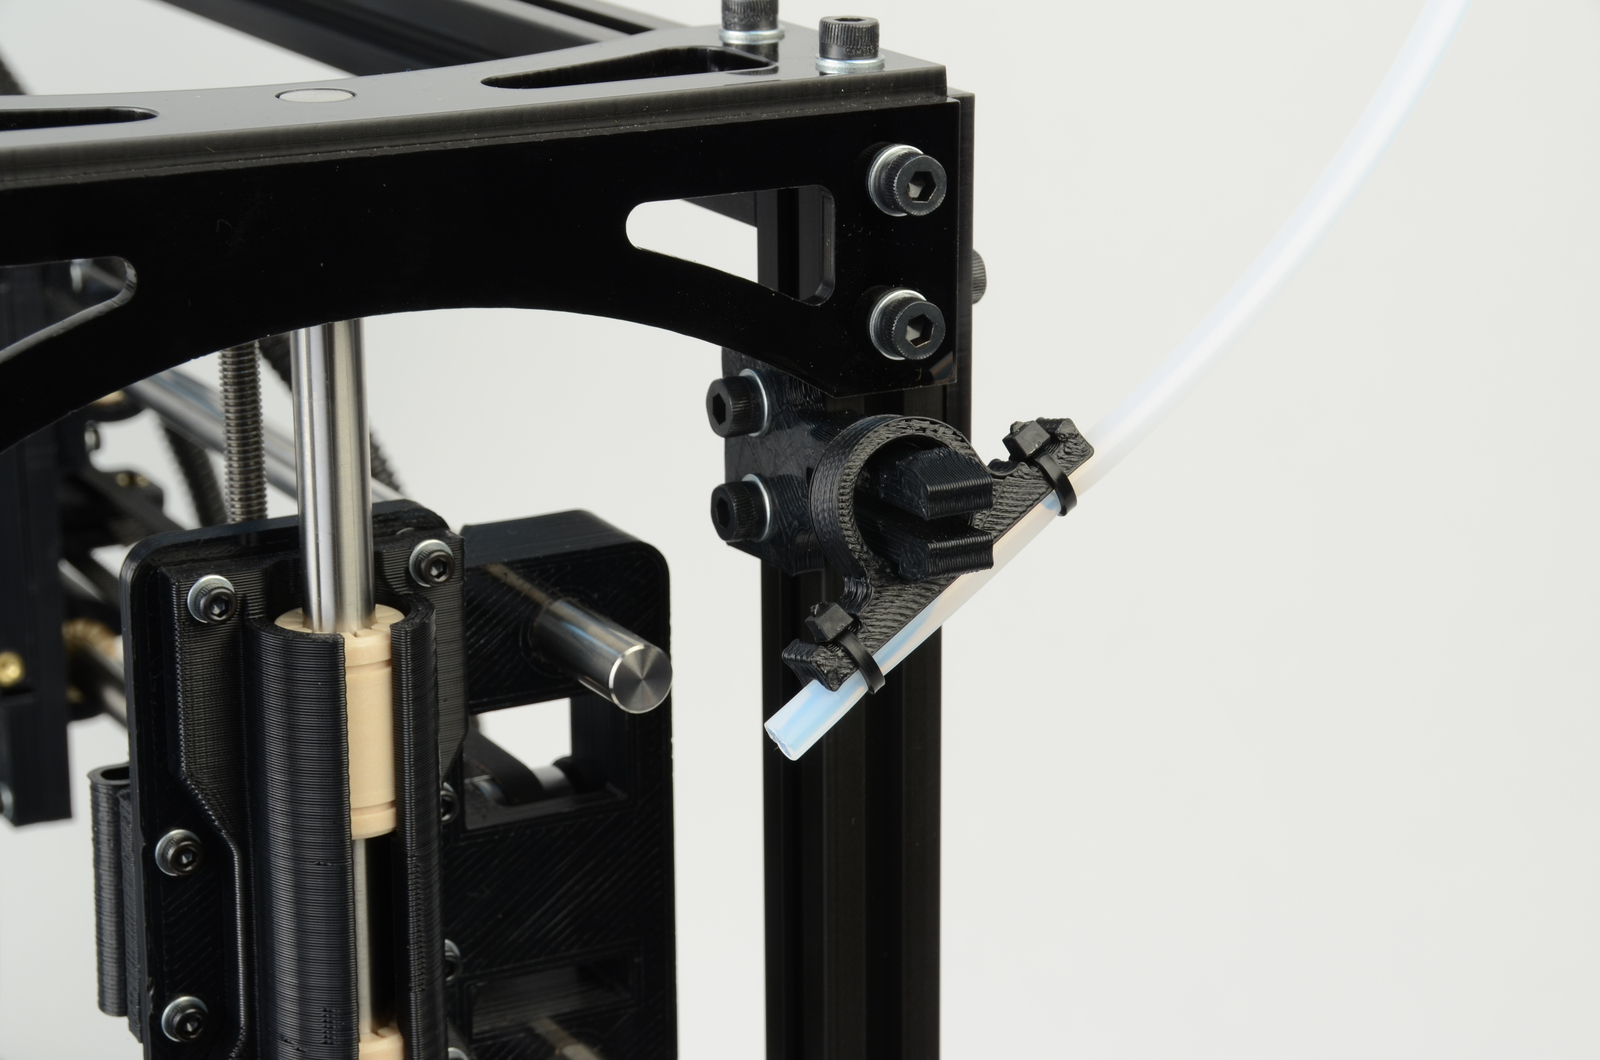
\includegraphics[keepaspectratio=true,angle=0,height=0.4\textheight,width=1.0\textwidth]{filament_guide_mount.JPG}
\caption{Filament Guide Mount}
\label{fig:filament_guide_mount}
\end{figure}

%\begin{figure}[hbt]
\begin{figure}[H]
\centering
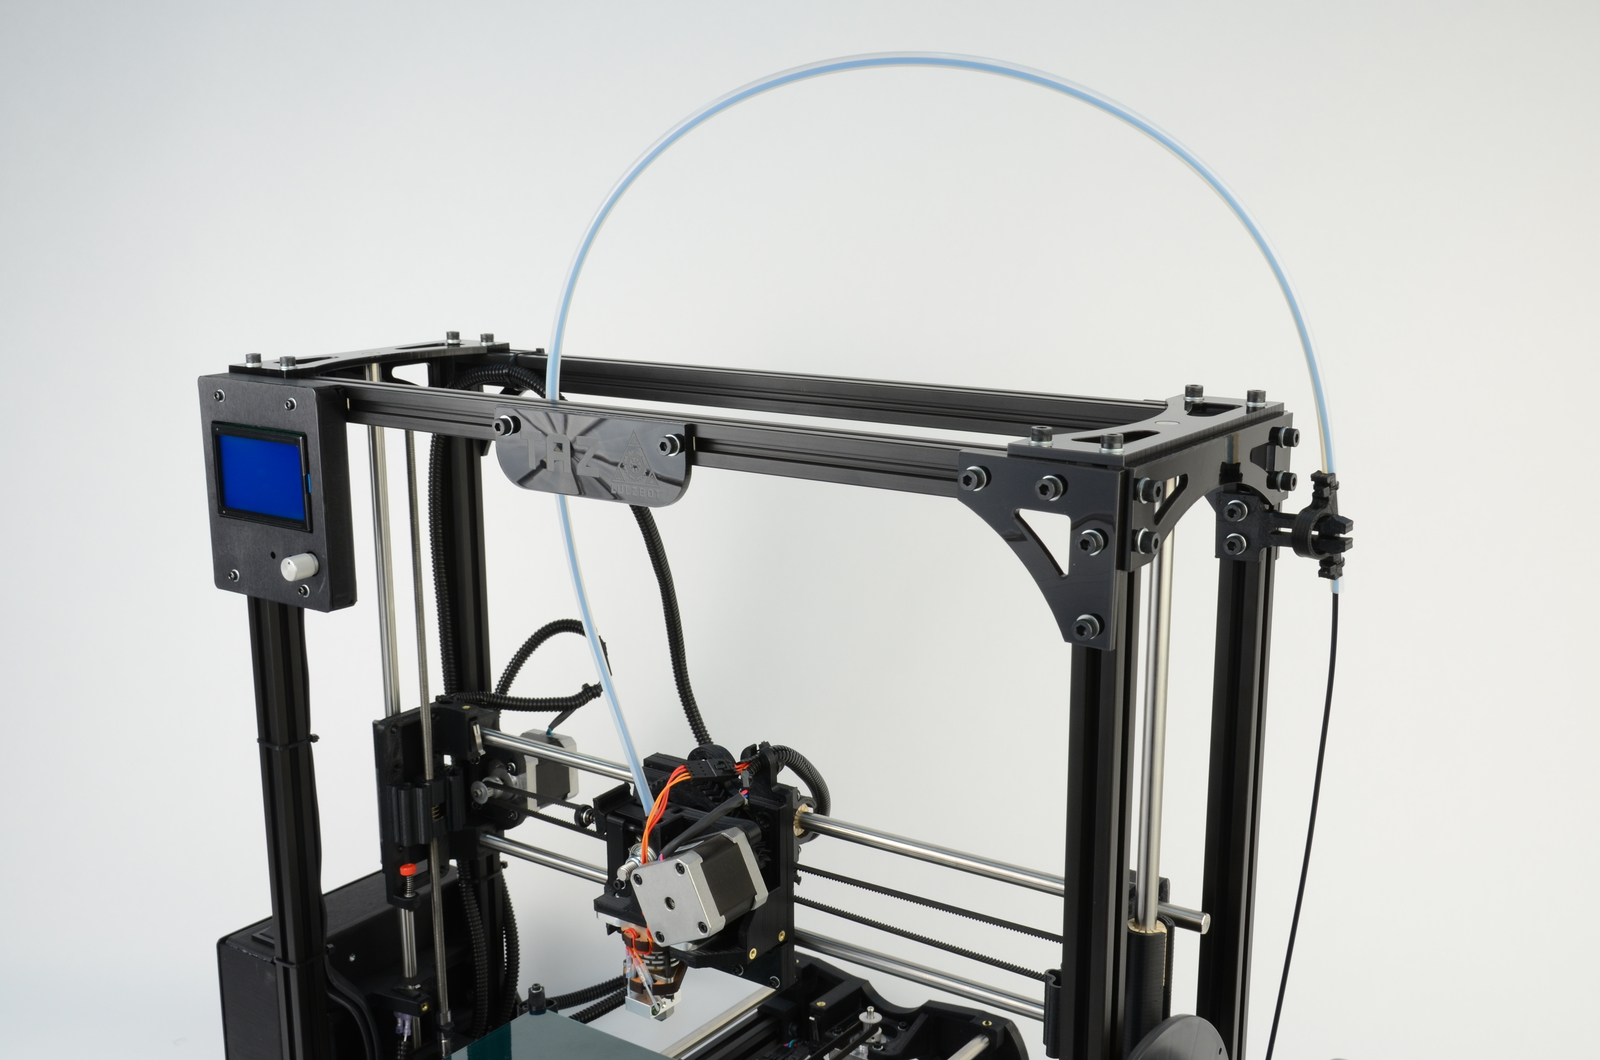
\includegraphics[keepaspectratio=true,angle=0,height=0.4\textheight,width=1.0\textwidth]{filament_guide_direction.JPG}
\caption{Filament Guide Setting}
\label{fig:filament_guide_setting}
\end{figure}

\index{end stops}
\glossary{End stops}{Mechanical or optical switches that are used to mark the 3 home (zero) positions.}
%\begin{figure}[hbt]
\begin{figure}[H]
\centering
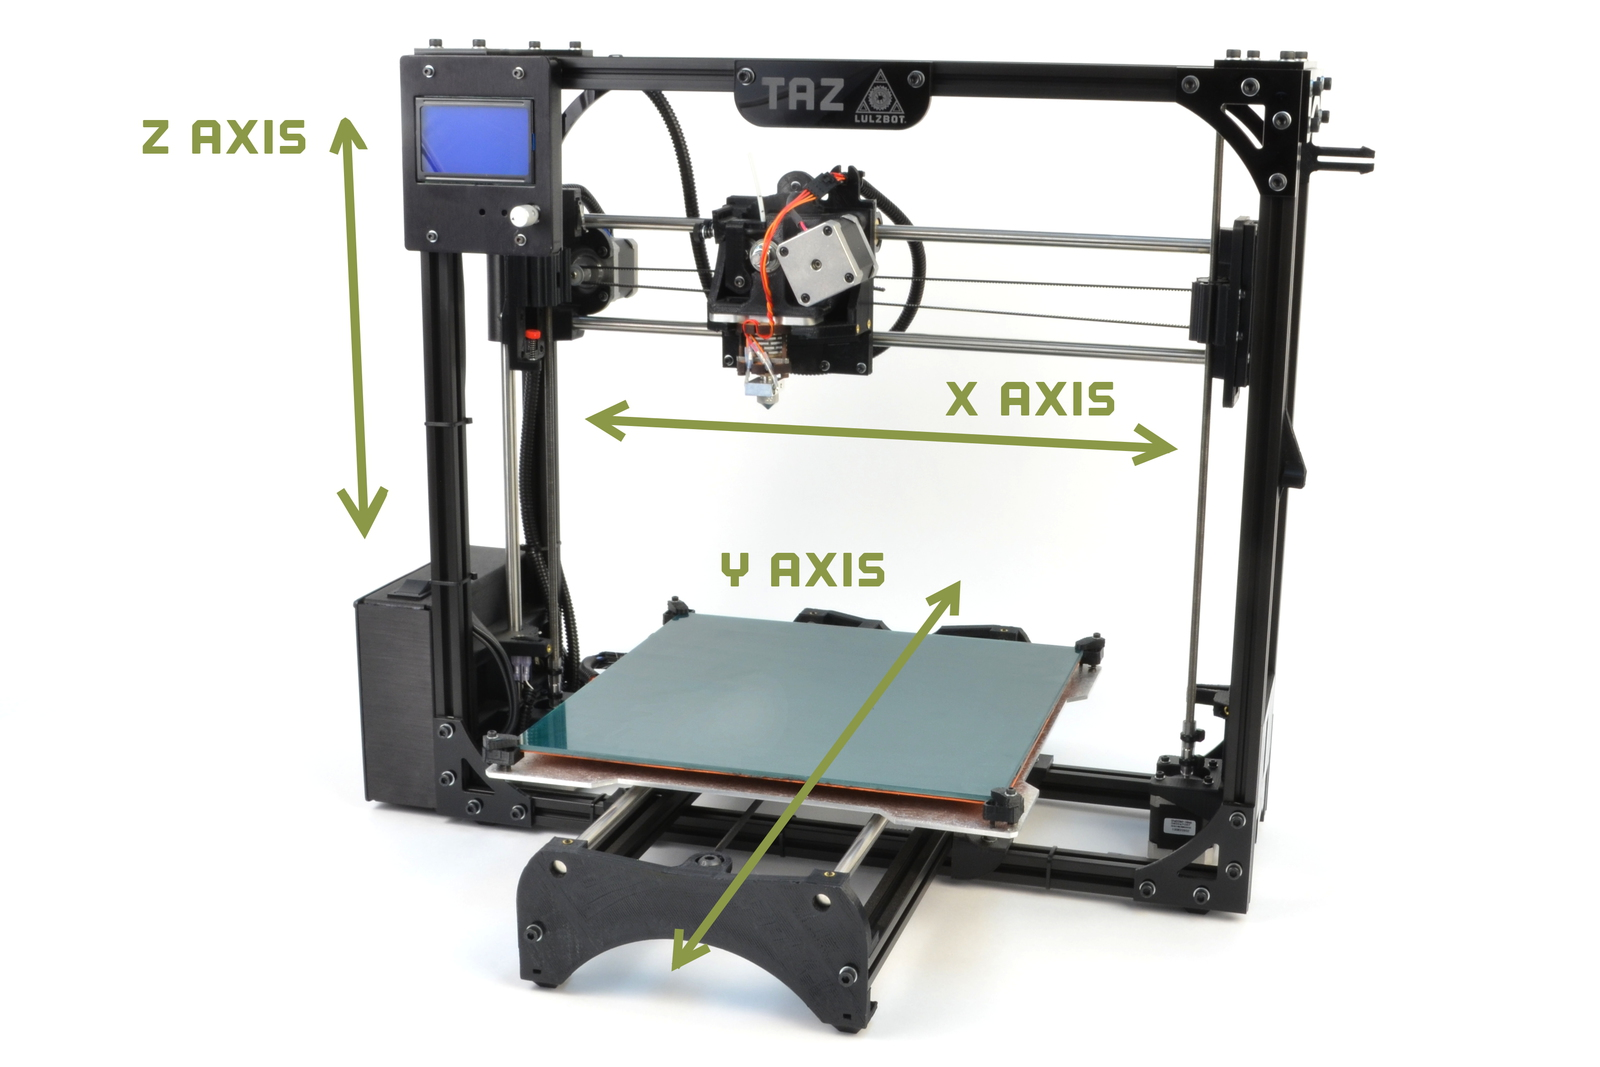
\includegraphics[keepaspectratio=true,angle=0,height=0.4\textheight,width=1.0\textwidth]{axes.JPG}
\caption{Axes movement directions}
\label{fig:axes_2}
\end{figure}

\begin{figure}[H]
\centering
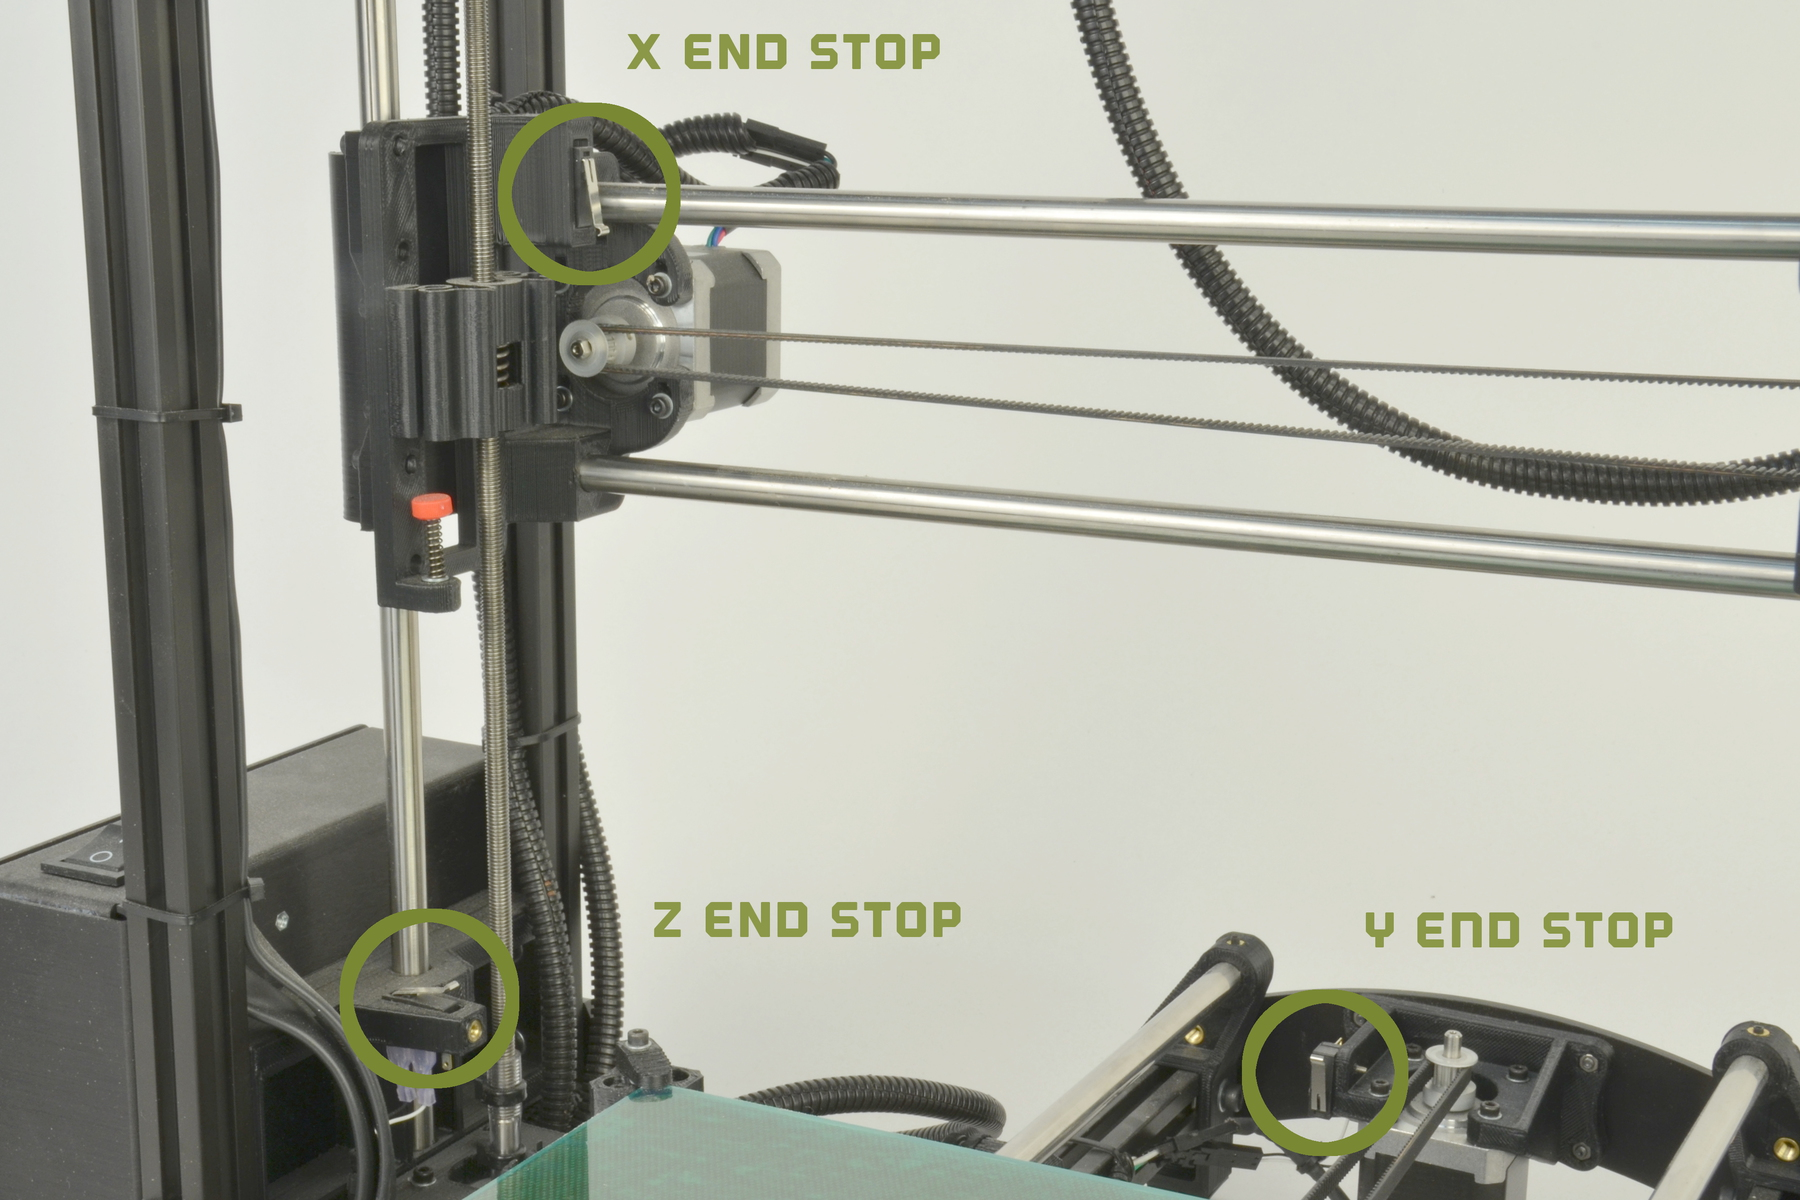
\includegraphics[keepaspectratio=true,angle=0,height=0.4\textheight,width=1.0\textwidth]{end_stop_switches.JPG}
\caption{End stop locations}
\label{fig:endstops}
\end{figure}



\begin{comment}
\index{driver}
\section{Installing Drivers}
Linux and Mac OSX users will not need to install a driver to communicate with the Mini 3D printer. Windows users will. The drivers can be downloaded from \texttt{LulzBot.com/support/downloads}. A visual guide showing the driver installation process can be found in our download section as well.

\index{pronterface}
\index{Printrun}
\index{pronsole}
\index{plater}
\index{stl}
\section{Installing Printrun}
Printrun contains several different applications that can be used to control the Mini 3D printer. It can be installed on Windows, Mac OSX and Linux based computers. Most users will use Pronterface, the graphical user interface for Printrun, when using a host software to interact with the 3D printer. \texttt{Pronsole} allows printing from the command line, and can be used for scripting and some automation. \texttt{Plater} allows you to arrange and combine several STL files into one. More information on the other programs within the Printrun package can be found at \texttt{https://github.com/kliment/Printrun}. Printrun can be downloaded from \texttt{LulzBot.com/support/downloads}. Download the version for your operating system and extract. You will need an archive manager to extract the files. If you do not have one installed we recommend using 7-zip, which can be downloaded for free at \texttt{www.1-zip.org}.

\begin{itemize}
\subsection{Windows Instructions}
\index{windows}
\item Once downloaded, extract the \texttt{dist} folder to a location of your choice. You can rename the \texttt{dist} folder if you like. Double click \texttt{pronterface.exe} to run Pronterface.


\subsection{Mac OSX Instructions}
\item Once downloaded, extract the \texttt{dist} folder to a location of your choice. Once extracted, double click the \texttt{pronterface-mac-Mar2012.app} file to install.

\subsection{Linux Instructions}
%\begin{itemize}
\item Once downloaded, extract the \texttt{dist} folder to a location of your choice. You will need to ensure that the following dependencies are met. They are listed in the README.md file. You can use this command to install the dependencies: 
\texttt{sudo apt-get install python-serial python-wxgtk2.8 python-pyglet python-tornado python-setuptools python-libxml2 python-gobject python-pip avahi-daemon libavahi-compat-libdnssd1}
followed by:
\texttt{pip install -r requirements.txt}
Open the \texttt{Printrun-source} folder in a terminal and enter the following command:
\texttt{sudo python setup.py install}.
Run Printrun by issuing the following command:
\texttt{python pronterface.py}
\end{itemize}

\index{Printrun}
\section{Using Printrun}

%\begin{figure}[hbt]
\begin{figure}[H]
\centering
\includegraphics[keepaspectratio=true,angle=0,height=0.4\textheight,width=1.0\textwidth]{Printrun.png}
\caption{Printrun}
\label{fig:Printrun}
\end{figure}

Printrun is used to control the printer from a computer. It is divided into 4 main parts: The buttons over the top are used to connect to the printer, load files and start \& stop prints.

The movement controls are on the left hand side, with the G-code preview window in the center and the Log window and Terminal command entry box on the right hand side (Fig. \ref{fig:Printrun_labels}, page \pageref{fig:Printrun_labels}).

\subsection{Connecting to the Mini 3D Printer}
To connect to the printer, select the correct port by using the drop down arrow and selecting the active port. The \texttt{Port} button will refresh the Port listing. Once selected choose the default \texttt{115200} buad rate and press \texttt{Connect}. Pronterface will open a connection to the printer and display firmware information in the Log window. If nothing is displayed in the Log window verify you have the correct port and connection speed selected. 

%\begin{figure}[hbt]
\begin{figure}[H]
\centering
\includegraphics[keepaspectratio=true,angle=0,height=0.4\textheight,width=1.0\textwidth]{Printrun-labels.png}
\caption{Printrun Functions}
\label{fig:Printrun-labels}
\end{figure}

\subsection{Movement} 
%\begin{figure}[hbt]
\begin{figure}[H]
\centering
\includegraphics[keepaspectratio=true,angle=0,height=0.4\textheight,width=1.0\textwidth]{Printrun_controls.png}
\caption{Movement Controls}
\label{fig:Printrun_controls}
\end{figure}

\subsubsection{Motors off}
The Mini 3D printer can be moved on all three axes independently. If you would like to do so by hand, use the \texttt{Motors off} button to unlock all the stepper motors. Once unlocked they can be moved by hand. Keep in mind that there is no positional feedback, so if you move an axis you will need to re-home in order to re-establish the hot end's position. 

\subsubsection{mm/min ZY:/ Z:}
These settings control the manual jog speeds when driven with Pronterface. Use caution when changing these figures. Moving the axes too fast can cause the printer to lose steps. If that occurs with the Z axis, it can potentially cause the Z axis to become out of square.

\subsubsection{Homing}
Each axes can be homed either individually or together. Press the \texttt{HomeX} button to move the X axis to the left until it activates the end stop. Once the X axis end stop is activated, the X axis carriage will 'bounce'- it will move over and move back to the home position more slowly. Press the \texttt{HomeY} button to home the Y axis. The Y axis platform will move away from you towards the rear of the printer. Press the \texttt{HomeZ} button to home the Z axis. The Z axis will move down towards the heated bed. Make sure that you home the printer immediately after power up. The printer will not know where the not end is until each axes has been homed. Moving prior to home can be risky since the 3D printer will not know it's initial location.  

\subsubsection{X/Y/Z Axes Movement Controls}
Prior to moving the X, Y or Z axis, make sure that you home each axis. The X, Y and Z axes can be moved utilizing the circular movement controls. Each axis can be moved in either fine moves or large moves, ranging from 0.1mm to 100mm.  For example, to move the \texttt{Y Axis} towards you, move your mouse to the \texttt{+y} section until both the \texttt{+y} and the \texttt{100} is highlighted then select that ring section. To move the \texttt{Y axis} away from you, move your mouse to the \texttt{-y} section until both the \texttt{-y} and the \texttt{100} is highlighted then select that ring section. The X axis can be moved in a similar fashion.

The Z axis movement control operates similarly, but the movement scale is different. The Z axis will move in 0.1mm, 1mm and 10mm increments. The top half of the movement bar will move the Z axis up, by the selected units, while the lower half will move the Z axis down, by the desired units. 
\end{comment}

\end{enumerate}
